\chapter{EIGEN VALUE PROBLEMS}
\section{Eigen Values and Eigen Function}
 The values of energy $E_n$ for which Schrodinger steady state equation can be solved are called eigen values and the corresponding wavefunctions $\psi_{n}$ are called eigen functions.\\
  The condition that a certain dynamical variable G be restricted to the descrete values $G_n$- in other words, that G be quandized-is that the wavefunction $\psi_{n}$ of the system be such that \\
  Eigen value equation $\implies \hat{G}\psi_{n}=G_n \psi_{n}$
  \section{Particle in a One Dimensional Box}
  \begin{figure}[H]
  	\centering
  	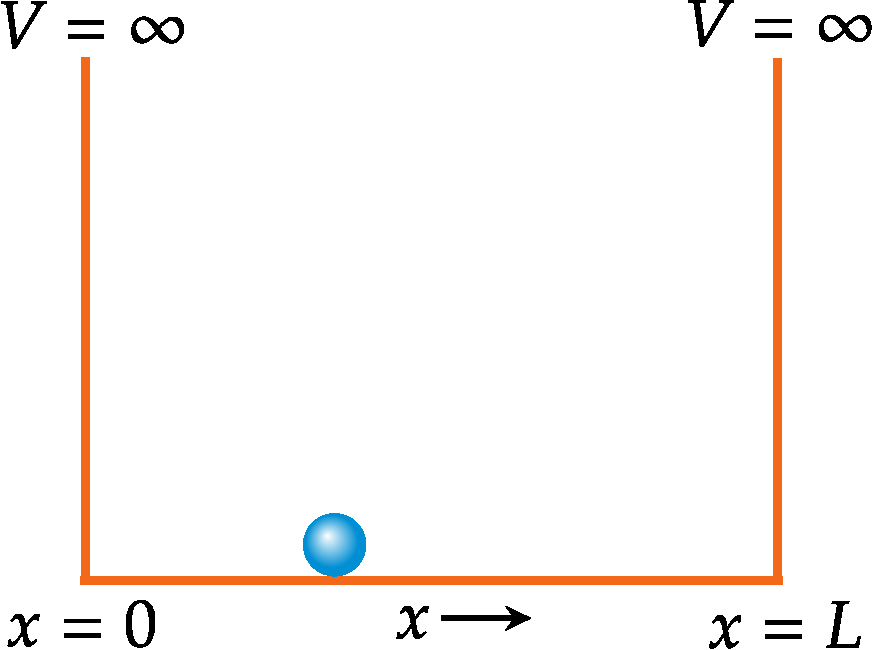
\includegraphics[height=4cm,width=5.5cm]{particle in abox}
  	\caption{Particle in a 1-D box}
  	\label{Particle in a 1-D box}
  \end{figure}
  Consider a particle of mass ' $m$ ' and energy ' $E$ ' is moving along $x$ -axis, in the region from $x=0$ to $x=L$ under the following potential i.e.
  \begin{equation}\label{key}
  V(x) = \begin{cases} 
  0 & 0<x<L  \\
  \infty & \text{Otherwise.}
  \end{cases}
  \end{equation}
  Here, the particle can move only on a line of finite length.The potential energy $V$ of the particle is infinite on both sides of the box, while $V$ is a constant-say $ 0 $ for convenience - on the inside (Figure.\ref{Particle in a 1-D box}. ). Because the particle cannot have an infinite amount of energy, it cannot exist outside the box, and so its wave function $\psi$ is $ 0 $ for $x \leq 0$ and $x \geq L$. Our task is to find what $\psi$ is within the box, namely, between $x=0$ and $x=L$.
  \begin{align}
  -\frac{\hbar^{2}}{2 m} \frac{d^{2} \psi(x)}{d x^{2}}+V \psi(x)&=E \psi(x)
  \intertext{Within the box Schrödinger's equation becomes,}
  -\frac{\hbar^{2}}{2 m} \frac{d^{2} \psi}{d x^{2}}&=E \psi \quad \text{Since, }\ V(x)=0\  \text{for} \ 0<x<L\\
  \frac{d^{2} \psi}{d x^{2}}+\frac{2 m}{\hbar^{2}} E \psi&=0\\
  \frac{d^{2} \psi}{d x^{2}}+k^{2} x&=0\qquad \text { Where, }\ k^{2}=\frac{2 m E}{\hbar^{2}}\label{particle1} 
  \intertext{The solution of the equation.\ref{particle1} can be written as, }
  \psi(x)&=A \sin k x+B \cos k x\\
  \psi&=A \sin \frac{\sqrt{2 m E}}{\hbar} x+B \cos \frac{\sqrt{2 m E}}{\hbar} x
  \end{align}
  \subsubsection{Boundary Conditions}
  $\psi(x)$ will be continuous at $x=0$ and $x=a$.
  \begin{enumerate}
  	\item Applying $\left.\psi(x)\right|_{x=0}=0 \quad \Rightarrow B=0$
  	\item Applying $\left.\psi(x)\right|_{x=L}=0 \quad \Rightarrow A \sin k L=0 \quad \Rightarrow k L=n \pi \Rightarrow k=\frac{n \pi}{L}$\\\\
  	$\Rightarrow \psi(x)=A \sin \left(\frac{n \pi {x}}{L}\right)\quad (n=1,2,3, \ldots \ldots \ldots)$ \ for\ $0<x<a$
  \end{enumerate}
  If $n=0 \Rightarrow k=0 \Rightarrow E=0 \Rightarrow \psi(x)=0$ everywhere inside the box. Therefore, there will be no admissible particle with zero energy within the box.
  \begin{center}
  	\framebox{
  		\parbox[t][2cm]{6cm}{
  			
  			\addvspace{0.2cm} \centering 
  			
  			\textbf{Particle in a one- dimensional box}\\ \vspace{0.3cm}
  			$\psi(x)=A \sin \left(\frac{n \pi {x}}{L}\right)$
  			
  	} }
  \end{center}
  \subsection{Normalisation of the Wavefunction of a Particle in a Box}
  The wave function $\psi_{n}$ corresponding to $\mathrm{n}^{\text {th }}$ quantum state is,
  \begin{equation}
  \psi(x) = \begin{cases} 
  A \sin \frac{n \pi x}{L} & 0<x<L  \\
  0 & \text{Otherwise.}
  \end{cases}
  \end{equation}
  Since, the particle must be somewhere within the box, the total probability of finding the particle inside the box is unity i.e.
  \begin{align}
  \int_{0}^{L} \psi_{n}^{*}(x) \psi_{n}(x) d x&=1 \\
  \int_{0}^{L} A^{2} \sin ^{2} \frac{n \pi x}{L} d x&=1\\
  A^{2} \int_{0}^{L} \frac{1}{2}\left[1-\cos \frac{2 \pi n x}{L}\right] d x&=1\\
  A&=\sqrt{\frac{2}{L}}
  \intertext{Therefore the normalised wave function of a particle in a one-dimensional box becomes,}
  \psi_{n}(x)&=\sqrt{\frac{2}{L}} \sin \left(\frac{n \pi x}{L}\right) \quad(n=1,2,3, \ldots \ldots \ldots \ldots \ldots)
  \end{align}
  \begin{center}
  	\framebox{
  		\parbox[t][2cm]{6cm}{
  			
  			\addvspace{0.2cm} \centering 
  			
  			\textbf{Wavefunction of a particle in a box} \\ \vspace{0.3cm}
  			$\psi_{n}(x)=\sqrt{\frac{2}{L}} \sin \left(\frac{n \pi x}{L}\right)$} }
  \end{center}
  \subsection{Energy of a Particle in a Box}
  We have found that the solution is subject to the boundary condition.  The sine term always yields $\psi=0$ at $x=0$, as required, but $\psi$ will be 0 at $x=L$ only when
  \begin{align}
  \frac{\sqrt{2 m E}}{\hbar} L&=n \pi \quad n=1,2,3, \ldots \label{particle2}
  \intertext{It is clear that the energy of the particle can have only certain values, solving equation.\ref{particle2},}
  E_{n}&=\frac{n^{2} \pi^{2} \hbar^{2}}{2 m L^{2}} \quad n=1,2,3, \ldots
  \end{align}
  \begin{center}
  	\framebox{
  		\parbox[t][2cm]{6cm}{
  			
  			\addvspace{0.2cm} \centering 
  			
  			\textbf{Energy of a particle in a box} \\ \vspace{0.3cm}
  			$E_{n}=\frac{n^{2} \pi^{2} \hbar^{2}}{2 m L^{2}}$ } }
  \end{center}
  So, we get an infinite sequence of descrete energy levels that corresponds to all integral values of $n$, where $n$ is called the quantum number representing the different states of the particle.
  \begin{align}
  \text{The ground state energy,} \quad E_{1}&=\frac{\pi^{2} \hbar^{2}}{2 m a^{2}}\\
  \text{The first excited state energy,} \quad 
  E_{2}&=\frac{4 \pi^{2} \hbar^{2}}{2 m a^{2}}\\
  \text{In general}\quad E_{n}&=n^{2} E_{1}
  \intertext{The difference in energy between two consecutive energy levels,}
  {\Delta E}_{n}&=E_{n+1}-E_{n}=\frac{\pi^{2} \hbar^{2}}{2 m a^{2}}\left[(n+1)^{2}-n^{2}\right]\\&=\frac{\pi^{2} \hbar^{2}}{2 m a^{2}}(2 n+1)
  \end{align}
  \begin{figure}[H]
  	\centering
  	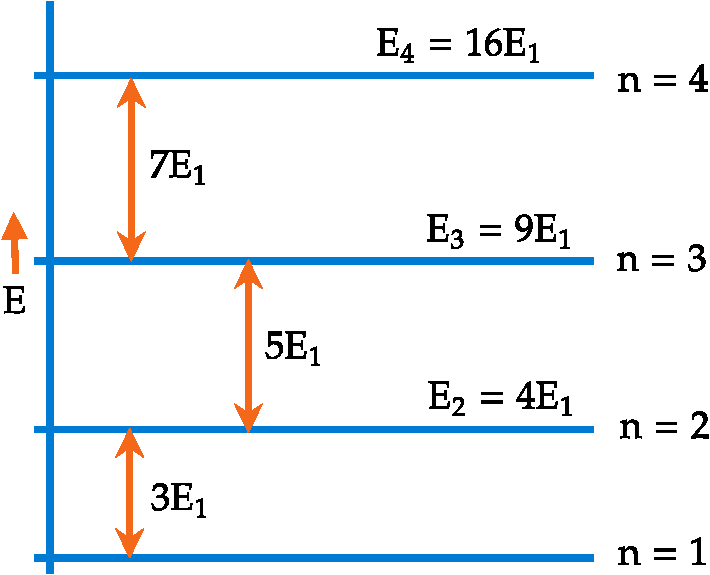
\includegraphics[height=5cm,width=6cm]{particle in a box1}
  	\caption{}
  	\label{}
  \end{figure}
  The normalized wave functions $\psi_{1}, \psi_{2}$, and $\psi_{3}$  the probability densities $\left|\psi_{1}\right|^{2},\left|\psi_{2}\right|^{2}$, and $\left|\psi_{3}\right|^{2}$ are plotted in Figure.\ref{Variation of wave function with eigen states.} and Figure.\ref{Variation of probability density with eigen states.} respectively, Although $\psi_{n}$ may be negative as well as positive, $\left|\psi_{n}\right|^{2}$ is never negative and, since $\psi_{n}$ is normalized, its value at a given $x$ is equal to the probability density of finding the particle there. In every case $\left|\psi_{n}\right|^{2}=0$ at $x=0$ and $x=L$, the boundaries of the box.
  \begin{figure}[H]
  	\begin{minipage}{0.30\textwidth}
  		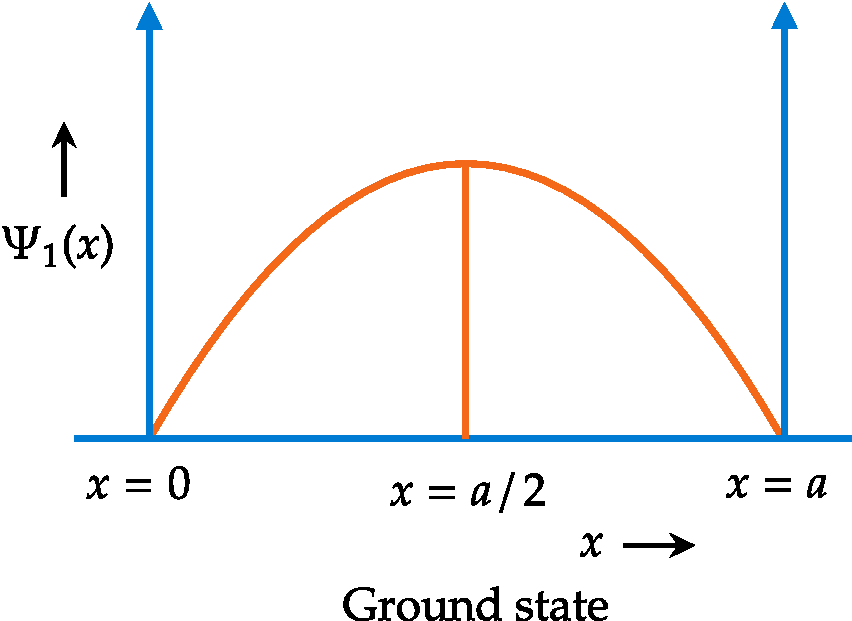
\includegraphics[height=3cm,width=4cm]{particle in a box5}
  	\end{minipage}
  	\begin{minipage}{0.30\textwidth}
  		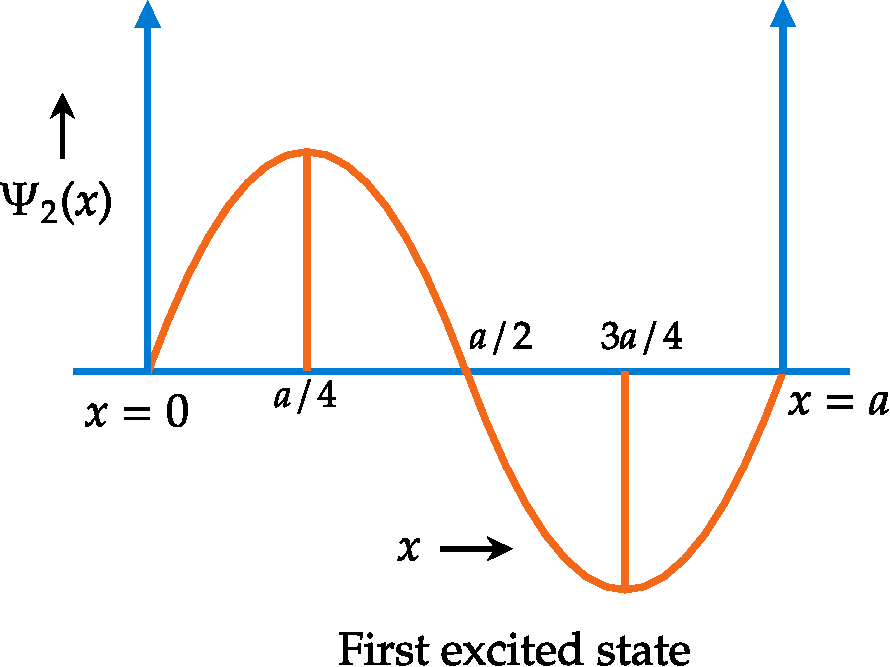
\includegraphics[height=3cm,width=4cm]{particle in a box6}
  	\end{minipage}
  	\begin{minipage}{0.30\textwidth}
  		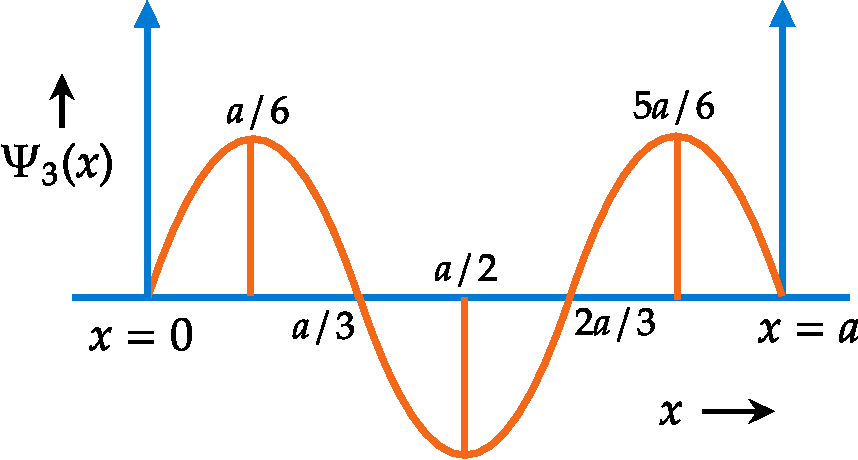
\includegraphics[height=3cm,width=4cm]{particle in a box7}
  	\end{minipage}
  	\caption{Variation of probability density with eigen states.}
  	\label{Variation of wave function with eigen states.}
  \end{figure}
  \begin{figure}[H]
  	\begin{minipage}{0.30\textwidth}
  		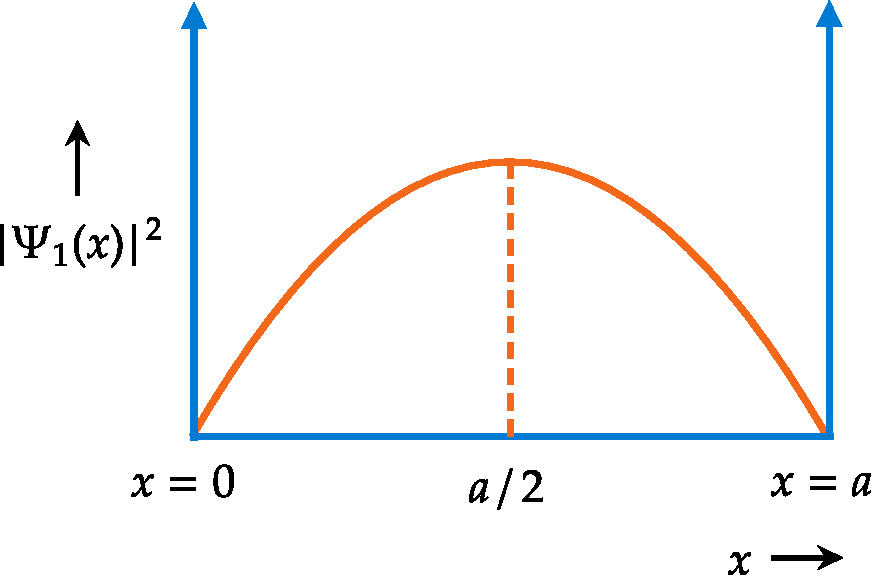
\includegraphics[height=3cm,width=4cm]{particle in a box3}
  	\end{minipage}
  	\begin{minipage}{0.30\textwidth}
  		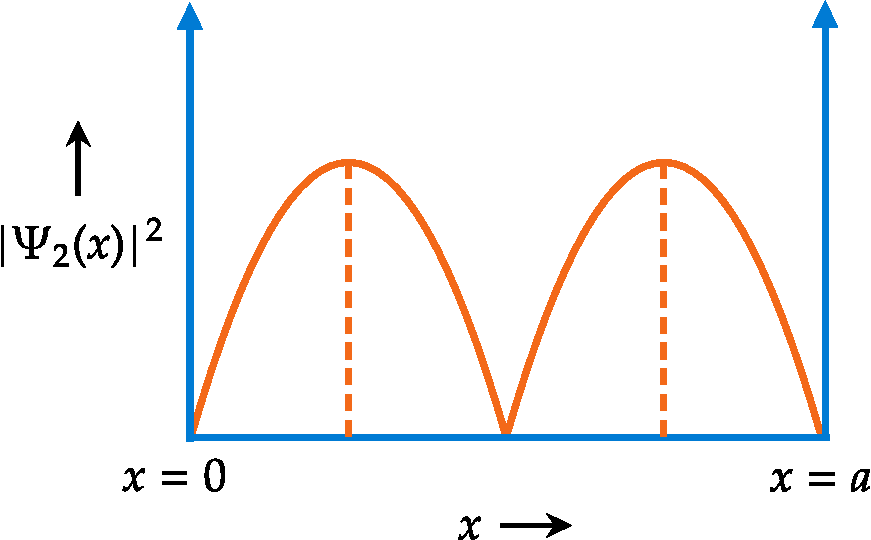
\includegraphics[height=3cm,width=4cm]{particle in a box2}
  	\end{minipage}
  	\begin{minipage}{0.30\textwidth}
  		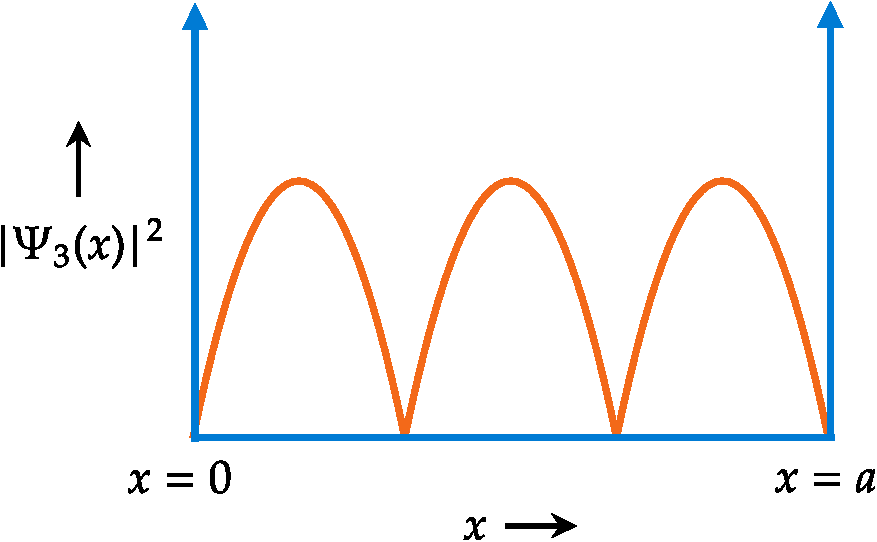
\includegraphics[height=3cm,width=4cm]{particle in a box4}
  	\end{minipage}
  	\caption{Variation of probability density with eigen states.}
  	\label{Variation of probability density with eigen states.}
  \end{figure}
  \section{Expectation Values of \Large{ $\hat{x}, \hat{p}_{x}, \hat{x}^{2}, \hat{p}_{x}^{2}$}}
  \subsection{Expectation Values of  Position \Large{ $\hat{x}$}}
  \begin{align*}
  \langle x\rangle &=\int_{-\infty}^{\infty} \psi^{*} x \psi =\int_{-\infty}^{\infty} x|\psi|^{2} d x=\frac{2}{L} \int_{0}^{L} x \sin ^{2} \frac{n \pi x}{L} d x \\
  &=\frac{2}{L}\left[\frac{x^{2}}{4}-\frac{x \sin (2 n \pi x / L)}{4 n \pi / L}-\frac{\cos (2 n \pi x / L)}{8(n \pi / L)^{2}}\right]_{0}^{L}
  \intertext{Since $\sin n \pi=0, \cos 2 n \pi=1$, and $\cos 0=1$, for all the values of $n$ the expectation value of $x$ is}
  \langle x\rangle&=\frac{2}{L}\left(\frac{L^{2}}{4}\right)\\&=\frac{L}{2}
  \end{align*}
  \subsection{Expectation Values of  Momentum \Large{$\hat{p_{x}}$}}
  \begin{align*}
  \langle p\rangle&=\int_{-\infty}^{\infty} \psi^{*} \hat{p} \psi d x\\&=\int_{-\infty}^{\infty} \psi^{*}\left(\frac{\hbar}{i} \frac{d}{d x}\right) \psi d x
  \intertext{Then we have to find the derivative of the wavefunction $\psi$}
  \psi^{*} &=\psi_{n}=\sqrt{\frac{2}{L}} \sin \frac{n \pi x}{L} \\
  \frac{d \psi}{d x} &=\sqrt{\frac{2}{L}} \frac{n \pi}{L} \cos \frac{n \pi x}{L}
  \intertext{Then ,}
  \langle p\rangle&=\frac{\hbar}{i} \frac{2}{L} \frac{n \pi}{L} \int_{0}^{L} \sin \frac{n \pi x}{L} \cos \frac{n \pi x}{L} d x\\&=\frac{\hbar}{i L}\left[\sin ^{2} \frac{n \pi x}{L}\right]_{0}^{L}\quad \text{Since,} \\
  &=0
  \intertext{The expectation value $\langle p\rangle$ of the particle's momentum is $0 .$}
  \intertext{In expectation value of momentum what we are realy determining is, the average value of the momentum .We know that the momentum eigenvalues of a particle in a box is given by,}
  p_{n}&=\pm \sqrt{2 m E_{n}}=\pm \frac{n \pi \hbar}{L} \quad (\text{Which is not equal to zero.})\\
  p_{\mathrm{av}}&=\frac{(+n \pi \hbar / L)+(-n \pi \hbar / \mathrm{L})}{2}\\&=0
  \end{align*}
  \subsection{Expectation Values of    \Large{$\hat{{x}}^{2}$}}
  \begin{align*}
  \left\langle x^{2}\right\rangle&=\int_{0}^{L} \psi^{*} x^{2} \psi d x\\&=\frac{2}{L} \int_{0}^{L} x^{2} \sin ^{2} \frac{n \pi x}{L} d x
  \\&=\frac{2}{L} \int_{0}^{L} x^{2}\left[ 1- \cos 2 \frac{n \pi x}{L}\right]  d x
  \\&=\frac{1}{L}\left[\left(\frac{x^{3}}{3}\right)_{0}^{L}-\left(x^{2} \frac{(\sin 2 n \pi x / L)}{(2 n \pi / L)}\right)_{0}^{L}+\int_{0}^{L} 2 x \cdot \sin \frac{(2 n \pi x / L)}{(2 n \pi / L)} d x\right]\\
  &=\frac{1}{L}\left[\frac{L ^{3}}{3}-0+2\left\{-x \frac{\cos \frac{2 n \pi x}{L}}{\left(\frac{2 n \pi}{L}\right)^{2}}+\frac{\sin \frac{2 n \pi x}{L}}{\left(\frac{2 n \pi}{L}\right)^{2}}\right\}_{0}^{L}\right]\\&=\frac{1}{L}\left[\frac{L^{3}}{3}-\frac{L^{3}}{2(n \pi)^{2}}\right]\\&=\frac{L^{2}}{3}-\frac{L^{2}}{2 n^{2} \pi^{2}}
  \end{align*}
  \subsection{Expectation Values of \Large{$\hat{{p_{x}}}^{2}$}}
  \begin{align*}
  \left\langle p^{2}\right\rangle&=\frac{2}{L} \int_{0}^{a} \sin \left(\frac{n \pi x}{a}\right)\left(-\hbar^{2} \frac{\partial^{2}}{\partial x^{2}}\right) \sin \left(\frac{n \pi x}{L}\right) d x\\&=\frac{2}{L}\left(-\hbar^{2}\right)\left(\frac{n \pi}{L}\right)^{2}(-1) \int_{0}^{L} \sin ^{2}\left(\frac{n \pi x}{L}\right) d x\\
  &=\frac{2}{L}\left(-\hbar^{2}\right)\left(\frac{n \pi}{L}\right)^{2}(-1) \int_{0}^{L} \sin ^{2}\left(\frac{n \pi x}{a}\right) d x\\
  &=\frac{n^{2} \pi^{2} \hbar^{2}}{L^{2}} \int_{0}^{L}\left[1-\cos \left(\frac{2 n \pi x}{L}\right)\right] d x
  \\&=\frac{n^{2} \pi^{2} \hbar^{2}}{L^{3}} \left[  x-\frac{\sin \frac{2n\pi x}{L}}{\frac{2n\pi x}{L}}\right] _{0}^{L}\\&=\frac{n^{2} \pi^{2} \hbar^{2}}{L^{2}}
  \end{align*}
  \subsection{Uncertainty in Position and Momentum}
  {\textbf{Uncertainty in Position:}}
  \begin{align*}
  \Delta \mathrm{x}&=\left[\left\langle\mathrm{x}^{2}\right\rangle-\langle\mathrm{x}\rangle^{2}\right]^{1 / 2}\\&=\left[\frac{L^{2}}{3}-\frac{\mathrm{L}^{2}}{2 {\mathrm{n}}^{2} \pi^{2}}-\frac{{L}^{2}}{4}\right]^{1 / 2}\\
  &=\left[\frac{\mathrm{L}^{2}}{12}-\frac{\mathrm{L}^{2}}{2 \mathrm{n}^{2} \pi^{2}}\right]^{1 / 2}=L\left[  \frac{1}{12}-\frac{1}{2 \mathrm{n}^{2} \pi^{2}}\right]^{1 / 2} 
  \end{align*}
  {\textbf{Uncertainty in Momentum:}}
  \begin{align*}
  \Delta\mathrm{p}&=\left[\left\langle\mathrm{p}^{2}\right\rangle-\langle\mathrm{p}\rangle^{2}\right]^{1 / 2}\\&=\left[ \frac{n^{2} \pi^{2} \hbar^{2}}{L^{2}}-0\right]^{\frac{1}{2}} \\&=\frac{\mathrm{n} \pi \hbar}{\mathrm{L}}\\
  \intertext{Therefore, the uncertainty product,} \Delta \mathrm{x} \Delta \mathrm{p}&= L\left[  \frac{1}{12}-\frac{1}{2 \mathrm{n}^{2} \pi^{2}}\right]^{1 / 2}   \frac{n\hbar }{L}\\&=\mathrm{n} \pi \hbar\left[\frac{1}{12}-\frac{1}{2 \mathrm{n}^{2} \pi^{2}}\right]^{1 / 2}
  \intertext{For \ $  n=1 $ ,}
  \Delta \mathrm{x} \Delta \mathrm{p}&=1.136\left(\frac{\hbar}{2}\right) \geq \hbar / 2
  \end{align*}
  \subsection{Particle in a 2-D Box}
  Consider a free particle of mass ${m}$ confined to move non-relativistically in a two-dimensional potential box of sides $L_{x}$ and $L_{y}$ parallel to the $x$ and $y$ -axes respectively. Since the particle is free, the potential inside the box is $V(x, y, )=0$. So, the total energy of the particle inside the box is equal to it's kinetic energy which is always a positive quantity.
  \begin{align}
  \intertext{Since the particle is confined two move in 2- dimensions i.e. \ $x$\  and \ $y$\, the  wavefunction of the system can be represented as,}
  \psi&= \psi{({x,y})}= \psi(x) \psi(y)\\
  \intertext{The potential inside the box is given by,}
  V(x, y)&=\left\{\begin{array}{ll}
  0, & \text { For }\quad  0<x<L_{x}\ ;\ 0<y<L_{y}\\
  \infty & \text { Elsewhere } 
  \end{array}\right.\\
  \intertext{The schrodinger equation of the system,}
  \nabla^{2} \psi{({x,y})}+ \frac{2m}{\hbar^{2}} (E-V)&=0\\
  \nabla^{2} \psi{({x,y})}+ \frac{2m}{\hbar^{2}} E&=0\quad (\text{Since,} \quad V=0)\\
  \nabla^{2}=\frac{\partial^{2}}{\partial x^{2}}+ \frac{\partial^{2}}{\partial y^{2}} \quad &\text{And} \quad \psi{({x,y})}=X(x)Y(y) \\ \text{Then,}\quad
  \left( \frac{\partial^{2}}{\partial x^{2}}+ \frac{\partial^{2}}{\partial y^{2}}\right)   X(x)Y(y)+ \frac{2m}{\hbar^{2}} E&=0\\
  Y\frac{\partial^{2} X}{\partial x^{2}}+X\frac{\partial^{2} Y}{\partial y^{2}}+ \frac{2m}{\hbar^{2}} E&=0 \label{Particle 2-d}
  \intertext{Divide equation.\ref{Particle 2-d} by (XY) gives,}
  \frac{1}{X}\frac{\partial^{2} X}{\partial x^{2}}+\frac{1}{Y}\frac{\partial^{2} Y}{\partial y^{2}}+\frac{2m(E_{x}+E_{y})}{\hbar^{2}}&=0  \label{particle 2d-1}\\
  \intertext{Then,}\quad \frac{1}{X}\frac{\partial^{2} X}{\partial x^{2}}+\frac{2m(E_{x})}{\hbar^{2}}+\frac{1}{Y}\frac{\partial^{2} Y}{\partial y^{2}}+\frac{2m(E_{y})}{\hbar^{2}}&=0
  \intertext{The two terms must be equal to zero individually. Then,}
  \frac{1}{X}\frac{\partial^{2} X}{\partial x^{2}}+\frac{2m(E_{x})}{\hbar^{2}}&=0 \quad \text{And}\quad \frac{1}{Y}\frac{\partial^{2} Y}{\partial y^{2}}+\frac{2m(E_{y})}{\hbar^{2}}=0\\
  \frac{\partial^{2} X}{\partial x^{2}}+k_{x}^{2} X&=0 \quad \text{And}\quad \frac{\partial^{2} Y}{\partial y^{2}}+k_{y}^{2} Y=0\\
  \text{Where, }\quad k_{x}^{2}&={\frac{\sqrt{2mE_{x}}}{\hbar}}
  \intertext{The solutions of the above equations can be found as,}
  X=\sqrt{\frac{2}{L_{x}}}\sin{\frac{n_{x}\pi x}{L_{x}}} \quad &\text{And} \quad  Y=\sqrt{\frac{2}{L_{y}}}\sin{\frac{n_{y}\pi y}{L_{y}}}\\
  \text{Where, }\quad k_{x}=\frac{n_{x}\pi }{L_{x}} \quad &\text{And } \quad  k_{y}=\frac{n_{y}\pi}{L_{y}}\\
  \psi(x,y)&=\sqrt{\frac{2}{L_{x}}} \sqrt{\frac{2}{L_{y}}} \sin{\frac{n_{x}\pi x}{L_{x}}}\sin{\frac{n_{y}\pi y}{L_{y}}}
  \end{align}
  \subsection{Energy of a Particle in a 2D Box}
  \begin{alignat*}{2}
  \intertext{We know that the total kinetic  energy of the particle can be written as,}
  &\left. \right. &&E=E_{x}+E_{y}\\
  &\text{Where, } \quad && E_{x}= \frac{p_{x}^{2}}{2m} \quad \text{and} \quad E_{y}= \frac{p_{y}^{2}}{2m}\\
  &\text{But,} \quad  &&p_{x}= \frac{\hbar^{2} k_{x}^{2}}{2m} \quad \text{and}\quad  p_{y}= \frac{\hbar^{2} k_{y}^{2}}{2m}\\
  &\text{Then,} \quad  &&E_{x}=\frac{{ n_{x}^{2}\hbar^{2}} {\pi}^{2}}{2m {L_{x}}^{2}} \quad \text{and}\quad E_{y}=\frac{{ n_{y}^{2}\hbar^{2}} {\pi}^{2}}{2m {L_{y}}^{2}}\\
  &\text{Or,} \quad &&E=  \frac{\hbar^{2}}{2m}\left(  k_{x}^{2}+k_{y}^{2}\right) \\
  &\text{Or,}\quad &&E= \frac{\hbar^{2} \pi^{2}}{2m}\left(  \frac{n_{x}^{2}}{L_{x}^{2}}+ \frac{n_{y}^{2}}{L_{y}^{2}}\right)
  \end{alignat*}
  \begin{center}
  	\framebox{
  		\parbox[t][2cm]{6cm}{
  			
  			\addvspace{0.2cm} \centering 
  			\textbf{Energy of a particle in 2-D box}\\ \vspace{0.2cm}
  			$E= \frac{\hbar^{2} \pi^{2}}{2m}\left(  \frac{n_{x}^{2}}{L_{x}^{2}}+ \frac{n_{y}^{2}}{L_{y}^{2}}\right)$} }
  \end{center}
  \subsubsection{Degeneracy of 2D Box}
  \begin{align*}
  \intertext{Energy of a particle in 2-D box,}
  E&= \frac{\hbar^{2} \pi^{2}}{2m}\left(  \frac{n_{x}^{2}}{L_{x}^{2}}+ \frac{n_{y}^{2}}{L_{y}^{2}}\right)\\
  \text{Let,}\quad L_{x}&=L_{y}=L\\
  \text{Then,}\quad E&= \frac{\hbar^{2} \pi^{2}}{2mL^{2}}\left({n_{x}^{2}}+ {n_{y}^{2}}\right)\\
  \text{Where,}\quad n_{x}&=n_{y}=1,2,3\cdots\\\\
  \text{Degeneracy of 2-D box}\quad &= 1\quad 2 \quad 1 \quad 2 \quad 2 \quad 2 \cdots
  \end{align*}
  \begin{table}[H]
  	\centering
  	\arrayrulecolor{ocre}
  	\newcolumntype{P}[1]{>{\centering\arraybackslash}p{#1}}
  	\renewcommand*{\arraystretch}{1.2}
  	\begin{tabular}{|P{1cm}|P{1cm}|P{4cm}|P{3cm}|P{3cm}|}
  		\hline
  		\multicolumn{5}{|c|}{\textbf{Degeneracy of 2-D box}}\\\hline\hline
  		$\mathbf{n_{x}}$&$\mathbf{n_{y}}$&\textbf{Energy}-$\mathbf{\left({n_{x}^{2}}+ {n_{y}^{2}}+{n_{z}^{2}}\right)\varepsilon}$& $\mathbf{\psi(x,y,z)}$&\textbf{Degeneracy}\\\hline\hline
  		1&1&2$\varepsilon$&$\psi(1,1)$ &None \\\hline
  		1&2&5$\varepsilon$ &$\psi(1,2)$&\multirow{2}{*}{Two fold } \\\cline{1-4}
  		2&1&5$\varepsilon$ &$\psi(1,2)$&\\\hline
  		2&2&8$\varepsilon$ &$\psi(2,2)$&None\\\hline
  		1&3&10$\varepsilon$ &$\psi(1,3)$&\multirow{2}{*}{Two fold } \\\cline{1-4}
  		3&1&10$\varepsilon$ &$\psi(3,1)$&\\\hline
  		2&3&13$\varepsilon$ &$\psi(2,3)$&\multirow{2}{*}{Two fold } \\\cline{1-4}
  		3&2&13$\varepsilon$ &$\psi(3,2)$&\\\hline
  		1&4&17$\varepsilon$ &$\psi(1,4)$&\multirow{2}{*}{Two fold } \\\cline{1-4}
  		4&1&17$\varepsilon$ &$\psi(4,1)$&\\\hline
  	\end{tabular}
  \end{table}
  \subsection{Particle in a 3-D Box}
  The particle in a 3-D box problem can be solved in the same way as that of particle in a 3-D box. Consider a free particle of mass ${m}$ confined to move non-relativistically in a three-dimensional potential box of sides $L_{x}, L_{y}$ and $L_{z}$ parallel to the $x, y$ and $z$ -axes respectively. Since the particle is free, the potential inside the box is $V(x, y, z)=0$. So, the total energy of the particle inside the box is equal to it's kinetic energy which is always a positive quantity.
  \begin{align}
  \intertext{If $ v $ be the velocity, then the momentum of the particle $p=m v$ and it's energy,}
  E&=\frac{1}{2}{m v}^{2}=\frac{p^{2}}{2 m}
  \intertext{The potential inside the box is given by,}
  V(x, y, z)=&\left\{\begin{array}{ll}
  0, & \text { For }\quad  0<x<L_{x}, 0<y<L_{y}, 0<z<L_{z}\\
  \infty & \text { For } \quad x>L_{x}, \quad y>L_{y}, \quad z>L_{z}
  \end{array}\right.
  \intertext { The wave equation describing the motion of the particle can be writen as, }\\
  \hat{H} \psi&=-\frac{\hbar^{2}}{2 m} \nabla^{2} \psi=E \psi \\ \frac{\partial^{2} \psi}{\partial x^{2}}+\frac{\partial^{2} \psi}{\partial y^{2}}+\frac{\partial^{2} \psi}{\partial z^{2}}+\frac{2 m E}{\hbar^{2}} \psi&=0 \label{particle in 3d-3}
  \intertext{As $V(x, y, z)=\infty$\  at the boundaries and outside the box $\psi(x, y, z)=0$ at the boundaries and outside the potential box. The boundary conditions can be written as,}
  \left.\begin{array}{r}
  \psi(x, y, z)=0 \text { at } x=0 \text { and } x=a \\
  y=0 \text { and } y=b \\
  z=0 \text { and } z=c
  \end{array}\right\}
  \intertext{The solution of the equation can be written as,}
  \psi(x, y, z)&=X(x) Y(y) Z(z) \label{particle in 3d-4}
  \intertext{ When we substitute equation.\ref{particle in 3d-4} in \ref{particle in 3d-3}, we get,}
  Y Z \frac{d^{2} X}{d x^{2}}+Z X \frac{d^{2} Y}{d y^{2}}+X Y \frac{d^{2} Z}{d z^{2}}+\frac{2 m E}{\hbar^{2}} X Y Z&=0  \label{particle in 3d-5}
  \intertext{Dividing equation. \ref{particle in 3d-5} by (XYZ)\ we get,}
  \frac{1}{X} \frac{d^{2} X}{d x^{2}}+\frac{1}{Y} \frac{d^{2} Y}{d y^{2}}+\frac{1}{Z} \frac{d^{2} Z}{d z^{2}}+\frac{2 m E}{\hbar^{2}}&=0
  \intertext{If $v_{x}, y_{y}$ and $v_{z}$ be the component of velocity of the particle along the $x, y$ and $z$ -axes respectively, then the corresponding kinetic energies of the particle are,}
  E_{x}=\frac{1}{2} m v_{x}^{2}, \quad E_{y}&=\frac{1}{2} m v_{y}^{2} \ \text { And } E_{z}=\frac{1}{2} m v_{z}^{2}\\\\ \text { Such that, }\quad E&=E_{x}+E_{y}+E_{z}\\\\
  \left[\frac{1}{X} \frac{d^{2} X}{d x^{2}}+\frac{2 m E_{x}}{\hbar^{2}}\right]&+\left[\frac{1}{Y} \frac{d^{2} Y}{d y^{2}}+\frac{2 m E_{y}}{\hbar^{2}}\right]+\left[\frac{1}{Z} \frac{d^{2} Z}{d z^{2}}+\frac{2 m {E}_{z}}{ \hbar^{2}}\right]=0\\\\
  \frac{1}{X} \frac{d^{2} X}{d x^{2}}+\frac{2 m E_{x}}{\hbar^{2}} X=0 \quad &\text{and}\quad
  \frac{1}{Y} \frac{d^{2} Y}{d y^{2}}+\frac{2 m E_{y}}{\hbar^{2}} Y=0  \quad \text{and}\quad
  \frac{1}{Z} \frac{d^{2} Z}{d z^{2}}+\frac{2 m E_{z}}{\hbar^{2}} Z=0\\
  X(x)=A_{1} \sin k_{x} x+B_{1} \cos k_{x} x \ &\text { where }\ k_{x}=\frac{\sqrt{2 m E_{x}}}{\hbar}\\
  Y(y)=A_{2} \sin{k}_{{y}} y+B_{2} \cos k_{y} y  \ & \text { where }\ k_{y}=\frac{\sqrt{2 m E_{y}}}{\hbar}\\
  Z(z)=A_{3} \sin k_{z} z+B_{3} \cos k_{z} z  \ & \text { where }\ k_{z}=\frac{\sqrt{2 m E_{z}}}{\hbar}
  \intertext{Then the solution of the Schrodinger equation for the wavefunction becomes,}
  \psi(x,y,z)&=\sqrt{\frac{2}{L_{x}}} \sqrt{\frac{2}{L_{z}}} \sqrt{\frac{2}{L_{x}}}\sin{\frac{n_{x}\pi x}{L_{x}}}\sin{\frac{n_{y}\pi y}{L_{y}}}\sin{\frac{n_{z}\pi z}{L_{z}}}
  \end{align}
  \subsection{Energy of a Particle in a 3D Box}
  \begin{alignat*}{2}
  \intertext{We know that the total kinetic  energy of the particle can be written as,}
  &\left. \right. &&E=E_{x}+E_{y}+E_{z}\\
  &\text{Where, } \quad && E_{x}= \frac{p_{x}^{2}}{2m} \quad \text{and} \quad E_{y}= \frac{p_{y}^{2}}{2m}\quad \text{and} \quad E_{z}= \frac{p_{z}^{2}}{2m}\\
  &\text{But,} \quad  &&p_{x}= \frac{\hbar^{2} k_{x}^{2}}{2m} \quad \text{and}\quad  p_{y}= \frac{\hbar^{2} k_{y}^{2}}{2m}\quad \text{and}\quad  p_{z}= \frac{\hbar^{2} k_{z}^{2}}{2m}\\
  &\text{Then,} \quad  &&E_{x}=\frac{{ n_{x}^{2}\hbar^{2}} {\pi}^{2}}{2m {L_{x}}^{2}} \quad \text{and}\quad E_{y}=\frac{{ n_{y}^{2}\hbar^{2}} {\pi}^{2}}{2m {L_{y}}^{2}} \quad \text{and}\quad E_{z}=\frac{{ n_{z}^{2}\hbar^{2}} {\pi}^{2}}{2m {L_{z}}^{2}}\\
  &\text{Or,} \quad &&E=  \frac{\hbar^{2}}{2m}\left(  k_{x}^{2}+k_{y}^{2}+k_{z}^{2}\right) \\
  &\text{Or,}\quad &&E= \frac{\hbar^{2} \pi^{2}}{2m}\left(  \frac{n_{x}^{2}}{L_{x}^{2}}+ \frac{n_{y}^{2}}{L_{y}^{2}}+\frac{n_{z}^{2}}{L_{z}^{2}}\right)
  \end{alignat*}
  \begin{center}
  	\framebox{
  		\parbox[t][2cm]{6cm}{
  			
  			\addvspace{0.2cm} \centering 
  			\textbf{Energy of a particle in 3-D box}\\ \vspace{0.2cm}
  			$E= \frac{\hbar^{2} \pi^{2}}{2m}\left(  \frac{n_{x}^{2}}{L_{x}^{2}}+ \frac{n_{y}^{2}}{L_{y}^{2}} + \frac{n_{z}^{2}}{L_{z}^{2}}\right)$} }
  \end{center}
  \subsubsection{Degeneracy of 3-D Box}
  \begin{align*}
  \intertext{Energy of a particle in 3-D box,}
  E&= \frac{\hbar^{2} \pi^{2}}{2m}\left(  \frac{n_{x}^{2}}{L_{x}^{2}}+ \frac{n_{y}^{2}}{L_{y}^{2}}+\frac{n_{z}^{2}}{L_{z}^{2}}\right)\\
  \text{Let,}\quad L_{x}&=L_{y}=L_{z}=L\\
  \text{Then,}\quad E&= \frac{\hbar^{2} \pi^{2}}{2mL^{2}}\left({n_{x}^{2}}+ {n_{y}^{2}}+{n_{z}^{2}}\right)\\
  \text{Where,}\quad n_{x}&=n_{y}=n_{z}=1,2,3\cdots\\\\
  \text{Degeneracy of 3-D box}\quad &= 1\quad 3 \quad 3 \quad 3 \quad 3 \quad 6 \quad 3  \cdots
  \end{align*}
  
  
  \begin{table}[H]
  	\centering
  	\arrayrulecolor{ocre}
  	\newcolumntype{P}[1]{>{\centering\arraybackslash}p{#1}}
  	
  	\renewcommand*{\arraystretch}{1.2}
  	\begin{tabular}{|P{1cm}|P{1cm}|P{1cm}|P{2.5cm}|P{3cm}|P{3cm}|}
  		\hline
  		\multicolumn{6}{|c|}{\textbf{Degeneracy of 3-D box}}\\\hline\hline
  		$\mathbf{n_{x}}$&$\mathbf{n_{y}}$&$\mathbf{n_{z}}$& \textbf{Energy}\newline$\mathbf{\left({n_{x}^{2}}+ {n_{y}^{2}}+{n_{z}^{2}}\right)\varepsilon}$& $\mathbf{\psi(x,y,z)}$&\textbf{Degeneracy}\\\hline\hline
  		1&1&1&3$\varepsilon$&$\psi(1,1,1)$ &None \\\hline
  		1&1&2&6$\varepsilon$ &$\psi(1,1,2)$&\multirow{3}{*}{Three fold } \\\cline{1-5}
  		1&2&1&6$\varepsilon$ &$\psi(1,2,1)$&\\\cline{1-5}
  		2&1&1&6$\varepsilon$ &$\psi(2,1,1)$&\\\hline
  		1&2&2&9$\varepsilon$ &$\psi(1,1,3)$&\multirow{3}{*}{Three fold } \\\cline{1-5}
  		2&1&2&9$\varepsilon$ &$\psi(1,3,1)$&\\\cline{1-5}
  		2&2&1&9$\varepsilon$ &$\psi(3,1,1)$&\\\hline
  		1&1&3&11$\varepsilon$ &$\psi(1,1,3)$&\multirow{3}{*}{Three fold } \\\cline{1-5}
  		1&3&1&11$\varepsilon$ &$\psi(1,3,1)$&\\\cline{1-5}
  		3&1&1&11$\varepsilon$ &$\psi(3,1,1)$&\\\hline
  		2&2&2&12$\varepsilon$ &$\psi(2,2,2)$& None\\\hline
  		1&2&3&14$\varepsilon$ &$\psi(1,1,2)$&\multirow{6}{*}{Six fold } \\\cline{1-5}
  		2&1&3&14$\varepsilon$ &$\psi(1,2,1)$&\\\cline{1-5}
  		3&2&1&14$\varepsilon$ &$\psi(1,2,1)$&\\\cline{1-5}
  		3&1&2&14$\varepsilon$ &$\psi(1,2,1)$&\\\cline{1-5}
  		1&3&2&14$\varepsilon$ &$\psi(1,2,1)$&\\\cline{1-5}
  		2&3&1&14$\varepsilon$ &$\psi(1,2,1)$&\\\hline
  		3&2&2&17$\varepsilon$ &$\psi(1,1,3)$&\multirow{3}{*}{Three fold } \\\cline{1-5}
  		2&3&2&17$\varepsilon$ &$\psi(1,3,1)$&\\\cline{1-5}
  		2&2&3&17$\varepsilon$ &$\psi(3,1,1)$&\\\hline
  		
  		
  		
  	\end{tabular}
  \end{table}
  \begin{figure}[H]
  	\centering
  	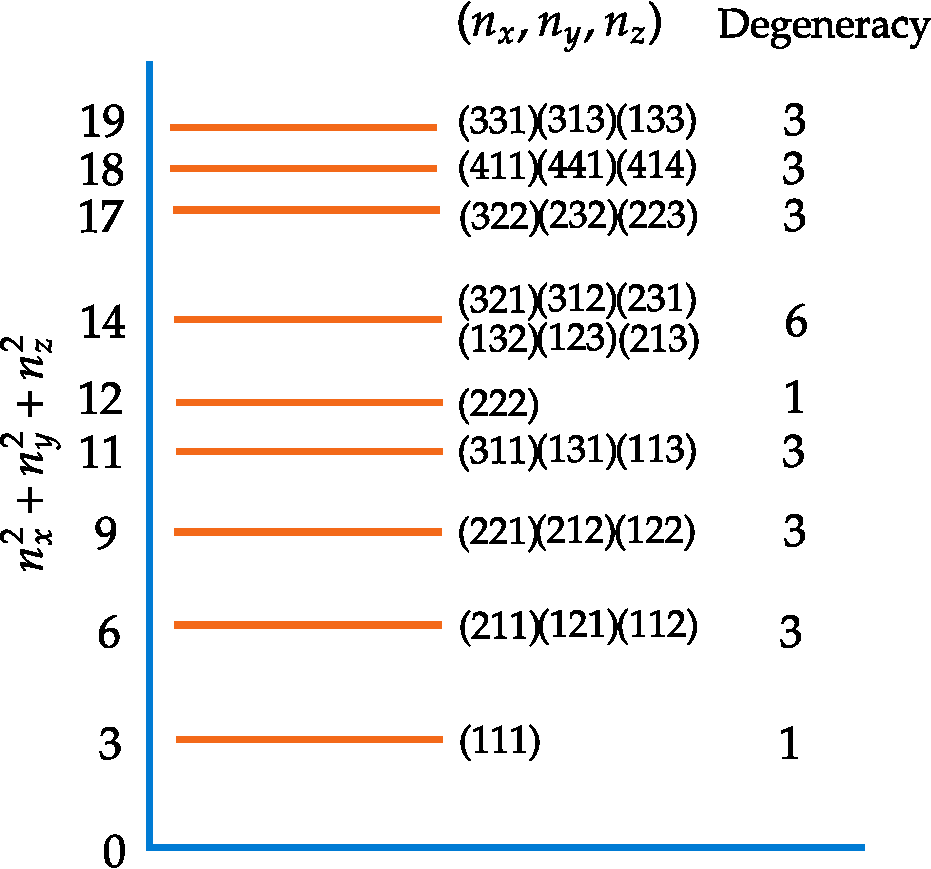
\includegraphics[height=7cm,width=7.5cm]{3D degeneracy}
  	\caption{Energy levels of 3D box}
  	\label{Energy levels of 3D box.}
  \end{figure}
\section{Finite Potential Well}

We have discussed potential wells with infinite potentials but in our real physical world 
Potential energies are never infinite , and the box with infinitely hard
walls  has no physical counterpart. However, potential wells
with barriers of finite height certainly do exist. Let us see what the wave functions and
energy levels of a particle in such a well are.
\begin{align*}
V(x)&=\left\{\begin{array}{ccc}
-V_{0}, & \text { For } & -L < x< L \\
0, & \text { For } & |x| \geq L
\end{array}\right.
\end{align*}
\begin{figure}[H]
	\centering
	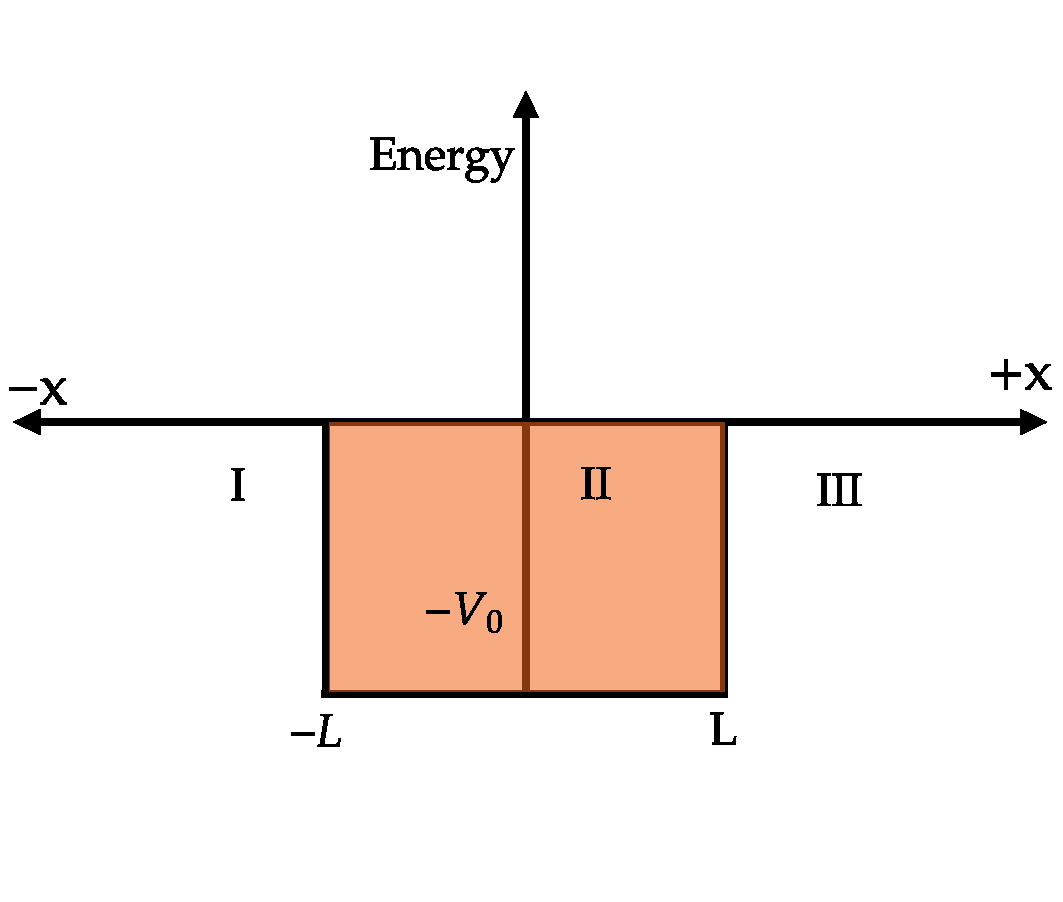
\includegraphics[height=7cm,width=9cm]{finite squre well}
	\caption{Finite potential well}
	\label{}
\end{figure}

The potential energy is zero for $|x|>a$. The potential energy is negative and equal to $-V_{0}$ in the well, because we defined $V_{0}$ to be a positive number. The width of the well is $2 a$.The width of the well is $2 a$.
entering regions $ I $ and $ III $. In quantum mechanics, the particle also bounces back and forth, but now it has a certain probability of penetrating into regions ${I}$ and $ III $ even though $E<U$. In regions $ I $ and $ III $ Schrödinger's steady-state equation is.
\begin{align}
\intertext{We have to find the Schrodinger equation in the potential well in the regions I,II and I. The schrodinger equation In regions I,}
\frac{d^{2} \psi_{I}}{d x^{2}}+\frac{2 m}{\hbar^{2}}(E-V) \psi_{I}&=0\\
\frac{d^{2} \psi_{I}}{d x^{2}}-\frac{2 m}{\hbar^{2}}(V-E) \psi_{I}&=0\\
D^{2}-K_{1}^{2}&=0\\
D&=\pm K_{1}\\\text{Then the wavefunction,}\quad  \psi_{I}&=A e^{-K_{1}x} +B e^{K_{1}x}
\intertext{In regions II Schrödinger's steady-state equation is,}
\frac{d^{2} \psi_{II}}{d x^{2}}+\frac{2 m}{\hbar^{2}}(E-V) \psi_{II}&=0\\
\frac{d^{2} \psi_{II}}{d x^{2}}+\frac{2 m}{\hbar^{2}}E \psi_{II}&=0\\
D^{2}+K_{2}^{2}&=0\\
D&=\pm i K_{2}\\
\psi_{II}&=C\cos K_{2}x+D\sin K_{2}x
\intertext{The schrodinger equation In regions III,}
\frac{d^{2} \psi_{III}}{d x^{2}}-\frac{2 m}{\hbar^{2}}(V-E) \psi_{III}&=0\\
D^{2}-K_{1}^{2}&=0\\
D&=\pm K_{1}\\\text{Then the wavefunction,}\quad  \psi_{III}&=F e^{-K_{1}x} +G e^{K_{1}x}
\end{align}
\begin{align}
\intertext{Both $\psi_{I}$ and $\psi_{\mathrm{III}}$ must be finite everywhere. Since $e^{-K_{1} x} \rightarrow \infty$ as $x \rightarrow-\infty$ and $e^{K_{1} x} \rightarrow \infty$ as $x \rightarrow \infty$, the coefficients $A$ and $F$ must therefore be $0 .$ Hence we have,}
\psi_\mathrm{I} &=B e^{K_{1} x} \quad \text{And }\quad  \psi_{\mathrm{III}} =F e^{-K_{1} x}
\intertext{These wave functions decrease exponentially inside the barriers at the sides of the well. Within the well Schrödinger's equation is the same as that of in infinite potential well and its solution is again.}
\psi_{\mathrm{II}}&=C \sin \frac{\sqrt{2 m E}}{\hbar} x+D \cos \frac{\sqrt{2 m E}}{\hbar} x \label{finite potential well}
\intertext{Here we have to apply the following rigid boundary conditions. Since the potential is an even function we only need to apply boundary condition on one side of the potential. (Say, x>a , at the region III)}
\text { 1. }\left(\psi_{I}\right)_{x=0}\hspace{0.6cm} &=\left(\psi_{II}\right)_{x=0}\\
\text { 2. }\left(\frac{d \psi_{I}}{d x}\right)_{x=0}&=\left(\frac{d \psi_{II}}{d x}\right)_{x=0}
\intertext{Applying these boundary conditions to equation. \ref{finite potential well} we get,}
\intertext{The continuity of $\psi(x)$, at $x=L$, says}
F e^{-K_{1} L}&=D \cos (K_{2} L)\label{finite 2}
\intertext{And the continuity of $d \psi / d x$, says,}
-K_{1} F e^{-K_{1} a}&=-K_{2} D \sin (K_{2}L)\label{finite 3}
\intertext{Dividing equation \ref{finite 2} by equation \ref{finite 3}, we find that,}
K_{1}=K_{2} \tan (K_{2} L) 
\intertext{This is a formula for the allowed energies, since $K_{1}$ and $K_{2}$ are both functions of $E$. To solve for $E$, we first adopt some nicer notation: Let}
z \equiv K_{2} L, \quad \text { and } \quad z_{0} \equiv \frac{L}{\hbar} \sqrt{2 m V_{0}}
\end{align}
\section{Step Potential}
represent a particle undergoing scattering in some potential. Here we examine the step potential  defined by,
$$
V(x)=\left\{\begin{array}{ll}
0, & x<0 \\
V_{0}, & x \geq 0
\end{array}\right.
$$ 
Our solutions to the Schrödinger equation with this potential will be scattering states of definite energy $E .$ We can consider two cases: 
\begin{enumerate}
	\item $E>V_{0}$. 
	\item $E<V_{0}$.
\end{enumerate}
In both cases the wavefunction extends infinitely to the left and is non-normalizable.
\subsection{Step Potential With $E>V_{0}$.}
Let us begin with the case $E>V_{0}$.
\begin{align*}
\intertext{The potential in the region I ,\ $ V=0 $ ,}
\frac{d^{2} \psi_{I}}{d x^{2}}+\frac{2 m}{\hbar^{2}}(E-V) \psi_{\text{I}}&=0
\intertext{The  Schrödinger equation in the region can be written as,}
\frac{d^{2} \psi_{\text{I}}}{d x^{2}}+\frac{2 m}{\hbar^{2}}E \psi_{\text{I}}&=0\\
D^{2}+ K_{1}^{2}&=0\\
D&=\pm iK_{1}\\
\psi_{\text{II}}&=Ae^{iK_{1}x}+Be^{-iK_{1}x}
\intertext{The potential in the region II ,\ $ V=V_{0} $ ,}
\intertext{The  Schrödinger equation in the region II can be written as,}
\frac{d^{2} \psi_{\text{II}}}{d x^{2}}+\frac{2 m}{\hbar^{2}}E \psi_{\text{II}}&=0\\
D^{2}+ K_{2}^{2}&=0\\
D&=\pm iK_{2}\\
\psi_{\text{II}}&=Ce^{iK_{2}x}+De^{-iK_{2}x}
\end{align*}
\subsection{Tunnel Effect}
Although the walls of the potential well were of finite height, they were assumed to be infinitely thick. As a result the particle was trapped forever even though it could penetrate the walls. We next look at the situation of a particle that strikes a potential barrier of height $U$, again with $E<\mathrm{U}$, but here the barrier has a finite width. What we will find is that the particle has a certain probability not necessarily great, but not zero either of passing through the barrier and emerging on the other side.
\section{The Potential Barrier}
Consider a beam of particle of mass m that are sent from the left on the potential barrier\\
$V(x)= \begin{cases}0, & x<0 \\ V_{0}, & 0 \leq x \leq a \\ 0, & x>a\end{cases}$
This potential, which is repulsive, supports no bound states. We are dealing here, as in the case of the potential step, with a one-dimensional scattering problem.

Again, let us consider the following two cases which correspond to the particle energies being respectively larger and smaller than the potential barrier.\\
\begin{figure}[H]
	\centering
	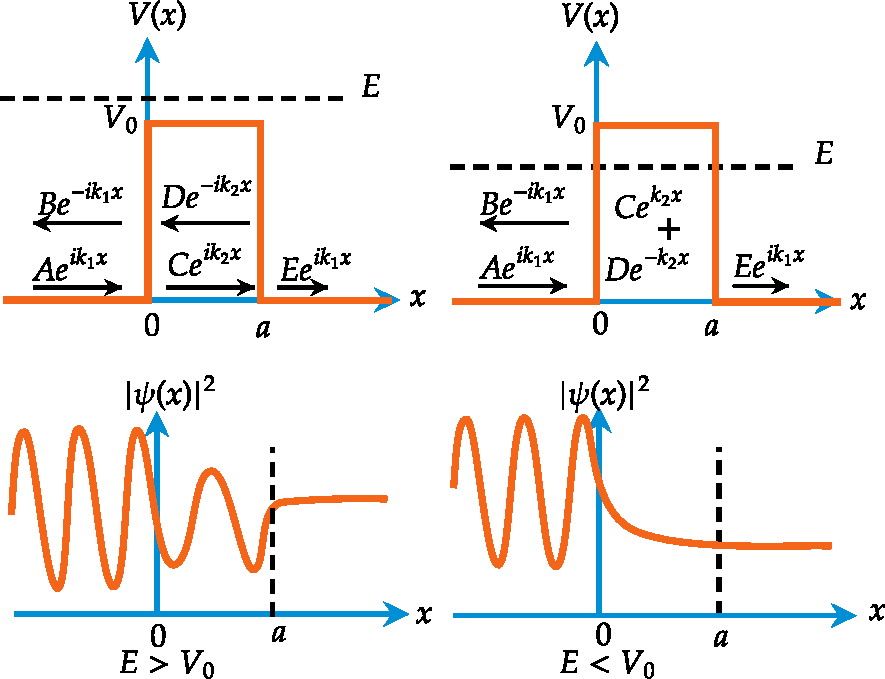
\includegraphics[height=9cm,width=15cm]{diagram-20220112-crop}
	\caption{}
	\label{}
\end{figure}
\subsection{The Case $E>V_0$}
Classically ,the particle that approach the barrier from the left at constant momentum,$p_1=\sqrt{2mE}$,as they enter the region $0\leq x \leq a$ will slow down to a momentum $p_2=\sqrt{2m(E-V_0)}$.They will maintain the momentum $p_2$ until they reach the point $x=a$.Then as soon as they pass beyond the point $x=a$ they will accelerate to the momentum $p_3=\sqrt{2mE}$ and maintain this value in the entire region $x>a$.Since the particles have enough energy to cross the barrier none of the particle will be reflected back;all the particles will emerge on the right side of $x=a$:\textit{total transmission}\\
The wavefunction in three region can be written as 
$$\psi(x)= \begin{cases}\psi_{1}(x)=A e^{i k_{1} x}+B e^{-i k_{1} x}, & x \leq 0, \\ \psi_{2}(x)=C e^{i k_{2} x}+D e^{-i k_{2} x}, & 0<x<a, \\ \psi_{3}(x)=E e^{i k_{1} x}, & x \geq a,\end{cases}$$
where $k_{1}=\sqrt{2 m E / \hbar^{2}}$ and $k_{2}=\sqrt{2 m\left(E-V_{0}\right) / \hbar^{2}}$. The constants $B, C, D$, and $E$ can be obtained in terms of $A$ from the boundary conditions: $\psi(x)$ and $d \psi / d x$ must be continuous at $x=0$ and $x=a$, respectively:
$$\begin{aligned}
	&\psi_{1}(0)=\psi_{2}(0), \quad \frac{d \psi_{1}(0)}{d x}=\frac{d \psi_{2}(0)}{d x}, \\
	&\psi_{2}(a)=\psi_{3}(a), \quad \frac{d \psi_{2}(a)}{d x}=\frac{d \psi_{3}(a)}{d x} .
\end{aligned}$$
These equations yield
$$
\begin{aligned}
A+B &=C+D, \quad i k_{1}(A-B)=i k_{2}(C-D), \\
C e^{i k_{2} a}+D e^{-i k_{2} a} &=E e^{i k_{1} a}, \quad i k_{2}\left(C e^{i k_{2} a}-D e^{-i k_{2} a}\right)=i k_{1} E e^{i k_{1} a} .
\end{aligned}
$$
Solving for $E$, we obtain
$$
\begin{aligned}
E &=4 k_{1} k_{2} A e^{-i k_{1} a}\left[\left(k_{1}+k_{2}\right)^{2} e^{-i k_{2} a}-\left(k_{1}-k_{2}\right)^{2} e^{i k_{2} a}\right]^{-1} \\
&=4 k_{1} k_{2} A e^{-i k_{1} a}\left[4 k_{1} k_{2} \cos \left(k_{2} a\right)-2 i\left(k_{1}^{2}+k_{2}^{2}\right) \sin \left(k_{2} a\right)\right]^{-1} .
\end{aligned}
$$
The transmission coefficient is thus given by
$$
\begin{aligned}
T &=\frac{k_{1}|E|^{2}}{k_{1}|A|^{2}}=\left[1+\frac{1}{4}\left(\frac{k_{1}^{2}-k_{2}^{2}}{k_{1} k_{2}}\right)^{2} \sin ^{2}\left(k_{2} a\right)\right]^{-1} \\
&=\left[1+\frac{V_{0}^{2}}{4 E\left(E-V_{0}\right)} \sin ^{2}\left(a \sqrt{2 m I_{0} / \hbar^{2}} \sqrt{E / V_{0}-1}\right)\right]^{-1} .
\end{aligned}
$$
$$\left(\frac{k_{1}^{2}-k_{2}^{2}}{k_{1} k_{2}}\right)^{2}=\frac{V_{0}^{2}}{E\left(E-V_{0}\right)}$$
Using the notation $\lambda=a \sqrt{2 m V_{0} / \hbar^{2}}$ and $\varepsilon=E / V_{0}$, we can rewrite $T$ as
\begin{center}
	\framebox{
		\parbox[t][3cm]{3.5cm}{
			
			\addvspace{0.2cm} \centering
			
			\begin{align*}
			\begin{array}{lll}
			 $$
			 T=\left[1+\frac{1}{4 \varepsilon(\varepsilon-1)} \sin ^{2}(\lambda \sqrt{\varepsilon-1})\right]^{-1} .
			 $$
			\end{array}
			\end{align*}} }
\end{center}

Similarly, we can show that reflection coefficient R
\begin{center}
	\framebox{
		\parbox[t][3cm]{3.5cm}{
			
			\addvspace{0.2cm} \centering
			
			\begin{align*}
			\begin{array}{lll}
			 $$
			 R=\frac{\sin ^{2}(\lambda \sqrt{\varepsilon-1})}{4 \varepsilon(\varepsilon-1)+\sin ^{2}(\lambda \sqrt{\varepsilon-1})}=\left[1+\frac{4 \varepsilon(\varepsilon-1)}{\sin ^{2}(\lambda \sqrt{\varepsilon-1})}\right]^{-1} .
			 $$
			\end{array}
			\end{align*}} }
\end{center}
\subsection{The Case $E<V_0$:Tunneling}
We are now going to show that the quantum mechanical predictions differ sharply from their classical counterparts, for the wave function is not zero beyond the barrier. The solutions of the Schrödinger equation in the three regions yield expressions that are similar to (4.36) except that $\psi_{2}(x)=C e^{i k_{2} x}+D e^{-i k_{2} x}$ should be replaced with $\psi_{2}(x)=C e^{k_{2} x}+D e^{-k_{2} x}:$\\
$$\psi(x)= \begin{cases}\psi_{1}(x)=A e^{i k_{1} x}+B e^{-i k_{1} x}, & x \leq 0 \\ \psi_{2}(x)=C e^{k_{2} x}+D e^{-k_{2} x}, & 0<x<a \\ \psi_{3}(x)=E e^{i k_{1} x}, & x \geq a\end{cases}$$
where $k_{1}^{2}=2 m E / \hbar^{2}$ and $k_{2}^{2}=2 m\left(V_{0}-E\right) / \hbar^{2}$. The behavior of the probability density corresponding to this wave function is expected, as displayed in Figure, to be oscillatory in the regions $x<0$ and $x>a$, and exponentially decaying for $0 \leq x \leq a$.\\
To find the reflection and transmission coefficients,
$$
R=\frac{|B|^{2}}{|A|^{2}}, \quad T=\frac{|E|^{2}}{|A|^{2}},
$$
we need only to calculate $B$ and $E$ in terms of $A$. The continuity conditions of the wave function and its derivative at $x=0$ and $x=a$ yield
$$\begin{aligned}
	A+B &=C+D, \\
	i k_{1}(A-B) &=k_{2}(C-D), \\
	C e^{k_{2} a}+D e^{-k_{2} a} &=E e^{i k_{1} a}, \\
	k_{2}\left(C e^{k_{2} a}-D e^{-k_{2} a}\right) &=i k_{1} E e^{i k_{1} a} .
\end{aligned}$$
The last two equations lead to the following expressions for $C$ and $D$ :
$$
C=\frac{E}{2}\left(1+i \frac{k_{1}}{k_{2}}\right) e^{\left(i k_{1}-k_{2}\right) a}, \quad D=\frac{E}{2}\left(1-i \frac{k_{1}}{k_{2}}\right) e^{\left(i k_{1}+k_{2}\right) a} .
$$
From these equations we can deduce the expression for Reflection coefficient and transmission coefficients as\\
R in terms of T,\\
$$R=\frac{1}{4} T\left(\frac{k_{1}^{2}+k_{2}^{2}}{k_{1} k_{2}}\right)^{2} \sinh ^{2}\left(k_{2} a\right) $$
Where T is \\
$$T=\left[1+\frac{1}{4}\left(\frac{k_{1}^{2}+k_{2}^{2}}{k_{1} k_{2}}\right)^{2} \sinh ^{2}\left(k_{2} a\right)\right]^{-1} $$
Now since
$$
\left(\frac{k_{1}^{2}+k_{2}^{2}}{k_{1} k_{2}}\right)^{2}=\left(\frac{V_{0}}{\sqrt{E\left(V_{0}-E\right)}}\right)^{2}=\frac{V_{0}^{2}}{E\left(V_{0}-E\right)}
$$
Now R and T becomes\\
$$\begin{aligned}
	R &=\frac{1}{4} \frac{V_{0}^{2} T}{E\left(V_{0}-E\right)} \sinh ^{2}\left(\frac{a}{\hbar} \sqrt{2 m\left(V_{0}-E\right)}\right) \\
	T &=\left[1+\frac{1}{4} \frac{V_{0}^{2}}{E\left(V_{0}-E\right)} \sinh ^{2}\left(\frac{a}{\hbar} \sqrt{2 m\left(V_{0}-E\right)}\right)\right]^{-1},
\end{aligned}$$
\begin{center}
	\framebox{
		\parbox[t][3cm]{3.5cm}{
			
			\addvspace{0.2cm} \centering
			
			\begin{align*}
			\begin{array}{lll}
			 $$\begin{aligned}
			 R &=\frac{T}{4 \varepsilon(1-\varepsilon)} \sinh ^{2}(\lambda \sqrt{1-\varepsilon}) \\
			 T &=\left[1+\frac{1}{4 \varepsilon(1-\varepsilon)} \sinh ^{2}(\lambda \sqrt{1-\varepsilon})\right]^{-1}
			 \end{aligned}$$
			\end{array}
			\end{align*}} }
\end{center}
$\text { where } \lambda=a \sqrt{2 m V_{0} / \hbar^{2}} \text { and } \varepsilon=E / V_{0} \text {. }$\\
\textbf{Special Cases}
\begin{enumerate}
	\item  If $E \ll V_{0}$, hence $\varepsilon \ll 1$ or $\lambda \sqrt{1-\varepsilon} \gg 1$, we may approximate $\sinh (\lambda \sqrt{1-\varepsilon}) \simeq$ $\frac{1}{2} \exp (\lambda \sqrt{1-\varepsilon})$. We can thus show that the transmission coefficient becomes asymptotically equal to
	$$
	\begin{aligned}
	T & \simeq\left\{\frac{1}{4 \varepsilon(1-\varepsilon)}\left[\frac{1}{2} e^{2 \sqrt{1-\varepsilon}}\right]^{2}\right\}^{-1}=16 \varepsilon(1-\varepsilon) e^{-2 i \sqrt{1-\varepsilon}} \\
	&=\frac{16 E}{V_{0}}\left(1-\frac{E}{V_{0}}\right) e^{-(2 a / \hbar) \sqrt{2 m\left(V_{0}-E\right)}}
	\end{aligned}
	$$
	This shows that the transmission coefficient is not zero, as it would be classically, but has a finite value. So, quantum mechanically, there is a finite tunneling beyond the barrier, $x>a$.
	\item Taking the classical limit $\hbar \rightarrow 0$, the coefficients reduce to the classical result: $R \rightarrow 1$ and $T \rightarrow 0$.
\end{enumerate}














































\section{Harmonic Oscillator}
There are only a very few potentials for which the Schrodinger equation can be solved analytically. The most important of these is the potential of the harmonic oscillator.
$$
V(x)=\frac{1}{2} kx^{2}=\frac{1}{2} km\omega^{2}x^{2}
$$
because so many of the systems encountered in nuclear physics, condensed matter physics, and elementary particle physics can be treated, to a first approximation, as a set of coupled harmonic oscillators. As we know harmonic motion takes place when a system of some kind vibrates about an equilibrium configuration.
\subsection{Harmonic Oscillator-Classical Treatement}
In the special case of simple harmonic motion, the restoring force $F$ on a particle of mass $m$ is linear; that is, $F$ is proportional to the particle's displacement $x$ from its equilibrium position and in the opposite direction.
Newton's law of motion $F=m a$ is generally non-linear, since $F(x)$ is usually a nonlinear function of $x$. However, if $F$ depends linearly on $x$, it follows that the potential depends quadratically on $x$, which implies a harmonic oscillator. We can write the equation of motion as,
\begin{align}
F &\propto -x \Rightarrow  F =-k x \\
\intertext{The potential of a 1-dimensional harmonic potential can be written as,}
U(x)&=\frac{1}{2}k x^{2} \\ \text{But,}\ k&=m\omega^{2}\quad  \text{And} \ \omega= \sqrt{\frac{k}{m}}\quad \Rightarrow \quad  \nu=\frac{1}{2\pi}\sqrt{\frac{k}{m}}\quad (\text{Angular frequency})\\
U(x)&=\frac{1}{2}m\omega^{2} x^{2}
\intertext{According to  Newton's laws of motion,}
F&=m a\\
-k x&=m \frac{d^{2} x}{d t^{2}}\\
\frac{d^{2} x}{d t^{2}}+\frac{k}{m} x&=0\\
\frac{d^{2} x}{d t^{2}}+\omega^{2} x&=0\\
\intertext{The solution of the equation can be written as,}
x(t)&=A \cos (\omega t)+A \sin (\omega t)
\intertext{Applying initial conditions, the solution will become}
x(t)&=A \cos (\omega t+\phi) \text{Where $A$ is the amplitude  of the wave}
\end{align}
The value of $\phi$, the phase angle, depends upon what $x$ is at the time $t=0$ and on the direction of motion then. The importance of the simple harmonic oscillator in both classical and modern physics lies not in the strict adherence of actual restoring forces to Hooke's law, which is seldom true, but in the fact that these restoring forces reduce to Hooke's law for small displacements $x$. As a result, any system in which something executes small vibrations about an equilibrium position behaves very much like a simple harmonic oscillator.
\subsubsection{Total Energy of the System}
\begin{align}
\intertext{The kinetic energy of the system can be written as,}T&=\frac{1}{2} m\left(\frac{d x}{d t}\right)^{2}\\&=\frac{1}{2} m a^{2} \omega^{2} \cos ^{2}(\omega t+\phi)\\&=\frac{1}{2} m \omega^{2} a^{2}\left[1-\sin ^{2}(\omega t+\phi)\right]\\&=\frac{1}{2} m \omega^{2}\left(a^{2}-x^{2}\right)
\intertext{Therefore, the total energy of the particle at $x$ is,}
E&=K.E+P.E\\
&=\frac{1}{2} m \omega^{2}\left(a^{2}-x^{2}\right)+\frac{1}{2} m \omega^{2} x^{2}\\ E&=\frac{1}{2} m \omega^{2} a^{2} \quad \text{Which is a constant.}
\intertext{The total energy $E$ is proportional to $a^{2} .$ Classically, the particle can oscillate with any amplitude $a$ and as such the total energy increases with the increase of $a$.The potential energy, $V=\frac{1}{2} k x^{2}$ has a parabolic form figure signifying that the particle executes motion in a potential well of parabolic form.}\notag
\end{align}
\begin{figure}[H]
	\centering
	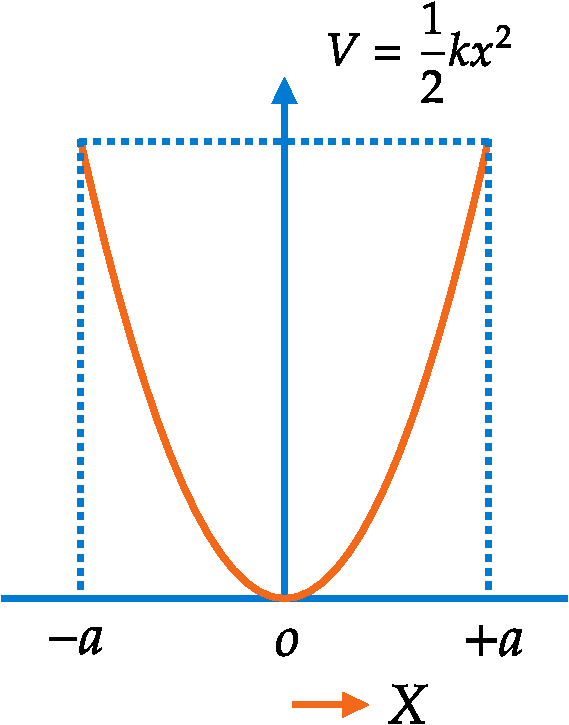
\includegraphics[height=6cm,width=5cm]{SHMclassical}
	\caption{The potential energy curve of Simple harmonic oscillator}
	\label{}
\end{figure}

\section{Harmonic Oscillator-Quantum Mechanical Treatment}
There are only a very few potentials for which the Schrodinger equation can be solved analytically. The most important of these is the potential of the harmonic oscillator.\\
The Hamiltonian of a particle of mass $m$ which oscillates with an angular frequency $\omega$ under the influence of a one-dimensional harmonic potential is\\
$$\hat{H}=\frac{\hat{P}^{2}}{2 m}+\frac{1}{2} m \omega^{2} \hat{X}^{2} $$
The problem is how to find the energy eigenvalues and eigenstates of this Hamiltonian. This problem can be studied by means of two separate methods. The first method, called the analytic method, consists in solving the time-independent Schrödinger equation (TISE) for the Hamiltonian. The second method, called the ladder or algebraic method, does not deal with solving the Schrödinger equation, but deals instead with operator algebra involving operators known as the creation and annihilation or ladder operators; this method is in essence a matrix formulation, because it expresses the various quantities in terms of matrices.
\subsection{Analytical Method}
\begin{align}
\intertext{The Schrodinger equation is given  by,}
\frac{d^{2} \psi}{d x^{2}}+\frac{2 m}{\hbar^{2}}\left(E-U\right) \psi&=0
\intertext{In the case of Harmonic oscillator, the potential energy, $U=\frac{1}{2}m\omega^{2}x^{2}$,}
\intertext{Then the Schrodinger equation becomes,}
\frac{-\hbar^{2}}{2 m}\frac{d^{2} \psi}{d x^{2}}+\frac{1}{2}m\omega^{2}x^{2} \psi&=E\psi
\intertext{The above differential equation is complex in form and thus need to be solved by Frobenious method. Then the general wavefunction of Harmonic oscillator can be found as,}
\psi_{n}(x)&=\left(\frac{\alpha}{2^{n}n!\sqrt{\pi}  }\right)^{1 / 2} e^{-\frac{1}{2}\alpha x^{2} } H_{n}({\alpha} x)
\intertext{Where $ H_{n}(\sqrt{\alpha} x)$\ is the Hermite polynomial.}
\text{For $n=0$}\quad \psi_{0}(x)&=\left(\frac{\alpha}{\pi}\right)^{1 / 4} e^{-\alpha x^{2} / 2}\\
\text{For $n=1$}\quad \psi_{1}(x)&=\left(\frac{\alpha}{2\sqrt{\pi}}\right)^{1 / 2} e^{-\alpha x^{2} / 2}(4(\alpha x)^{2}-2)\\
\end{align}
\begin{center}
	\framebox{
		\parbox[t][1cm]{8cm}{
			
			\addvspace{0.2cm} \centering 
			
			$\psi_{n}(x)=\left(\frac{\alpha}{2^{n}n!\sqrt{\pi}  }\right)^{1 / 2} e^{-\frac{1}{2}\alpha x^{2} } H_{n}({\alpha} x)$} }
\end{center}
\begin{figure}[H]
	\centering
	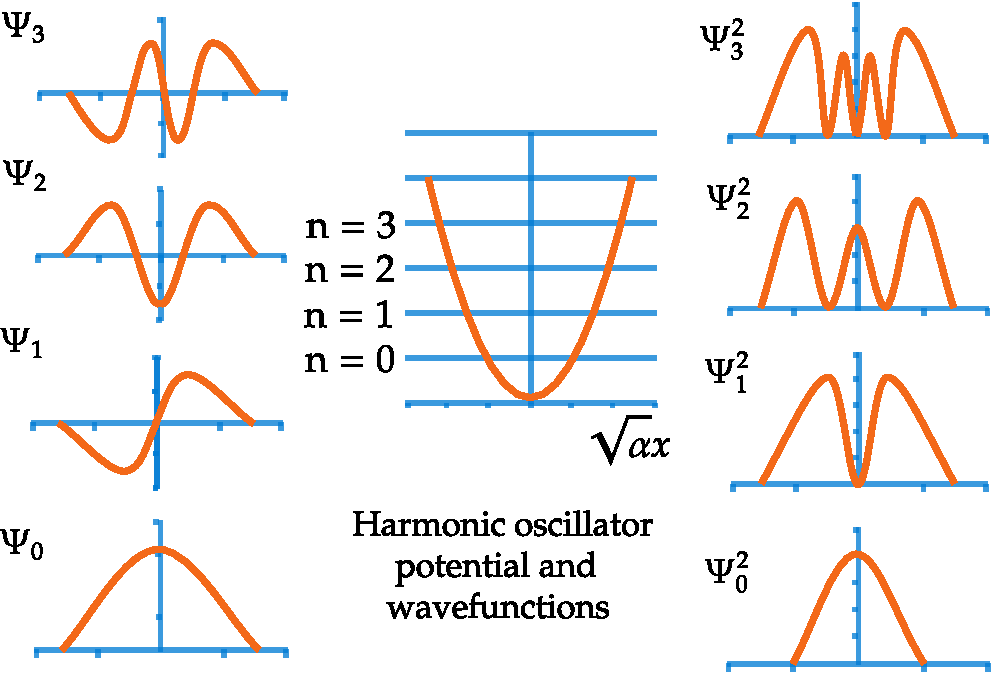
\includegraphics[height=7cm,width=10cm]{SHM1}
	\caption{Wavefunctions and Probability densities of Harmonic wavefunction}
	\label{ Harmonic wavefunction}
\end{figure}
\begin{note}
	\textbf{Hermite Polynomial Values}
	\begin{align*}
	H_{0}(x)&=1 \\
	H_{1}(x)&=2 x \\
	H_{2}(x)&=4 x^{2}-2 \\
	H_{3}(x)&=8 x^{3}-12 x \\
	H_{4}(x)&=16 x^{4}-48 x^{2}+12 \\
	H_{5}(x)&=32 x^{5}-160 x^{3}+120 x \\
	\end{align*}
\end{note}

\subsubsection{Energy levels of Harmonic oscillator}
The energy eigen values of the Harmonic oscillator is given by,
\begin{align*}
E_{n}&=(n+\frac{1}{2})\hbar \omega
\intertext{The energy eigen values at different states,}
\text{At \ $n=0$\ } \quad ; \quad & E_{0}=\frac{1}{2}\hbar \omega \quad (\text{i.e., The energy eigen value at ground state is not equal to zero.})\\
\text{At \ $n=1$\ } \quad ; \quad & E_{1}=\frac{3}{2}\hbar \omega\\
\text{At \ $n=2$\ } \quad ; \quad & E_{2}=\frac{5}{2}\hbar \omega\\
\text{At \ $n=3$\ } \quad ; \quad & E_{3}=\frac{7}{2}\hbar \omega\\
\end{align*}

\begin{figure}[H]
	\centering
	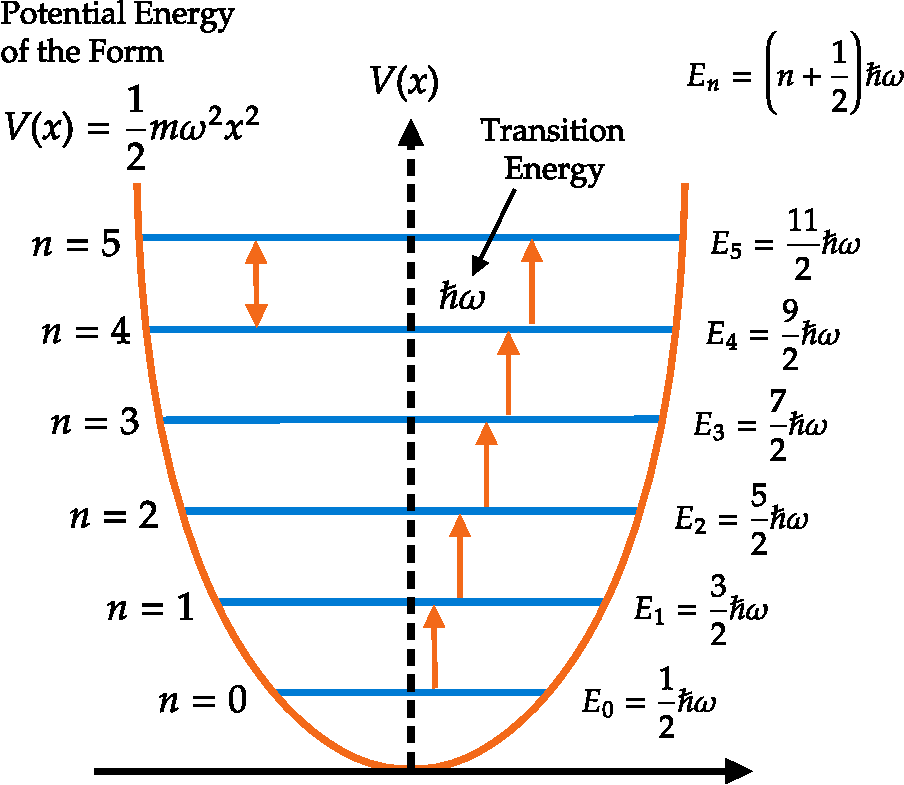
\includegraphics[height=8cm,width=9cm]{shm energy level}
	\caption{Energy levels of Harmonic Oscillator}
	\label{Energy levels of Harmonic Oscillator}
\end{figure}
\subsection{Algebraic method(ladder method)}
   Let us now show how to solve the harmonic oscillator eigen value problem using the algebraic method.For this we need to rewrite the hamiltonian interms of two hermitian dimensionless operators $\hat{p}=\hat{P}/\sqrt{m\hbar \omega}$ and $\hat{q}=\hat{X}\sqrt{m\omega/\hbar}$\\
   $$\hat{H}=\frac{\hbar \omega}{2}\left( \hat{p}^2+\hat{q}^2\right) $$
   And then introduce two non hermitian dimensioless operators:
   $$\hat{a=\frac{1}{\sqrt{2}}}(\hat{q}+i\hat{p}), \quad \quad \hat{a}^{\dagger}=\frac{1}{\sqrt{2}}(\hat{q}-i\hat{p})$$
   Note that $\hat{a}^{\dagger}\hat{a}=\frac{1}{2}(\hat{q}-i\hat{p})(\hat{q}+i\hat{p})=\frac{1}{2}\left( \hat{q}^2+\hat{p}^2+i\hat{q}\hat{p}-i\hat{p}\hat{q}\right) =\frac{1}{2}(\hat{q}^2+\hat{p}^2)+\frac{i}{2} \left[ \hat{q},\hat{p}\right] $\\\\
   Where using $ \left[ \hat{X}, \hat{P} \right] =i\hbar$, we can verify that the commuttator between $\hat{q}$ and $\hat{p}$ is \\
   $$\left[ \hat{q}, \hat{p}\right] =\left[ \sqrt{\frac{m\omega}{\hbar}}\hat{X},\frac{1}{\sqrt{\hbar m\omega}}\hat{P}\right]=\frac{1}{\hbar}\left[ \hat{X},\hat{P}\right] =i$$
   $$\begin{aligned}
   	&\hat{a}^{\dagger} \hat{a}=\frac{1}{2}\left(\hat{q}^{2}+\hat{p}^{2}\right)-\frac{1}{2} \\
   	&\frac{1}{2}\left(\hat{q}^{2}+\hat{p}^{2}\right)=\hat{a}^{\dagger} \hat{a}+\frac{1}{2}
   \end{aligned}$$
   Inserting this into Hamiltonian we will get \\
   $$\hat{H}=\hbar \omega\left(\hat{a}^{\dagger} \hat{a}+\frac{1}{2}\right)=\hbar \omega\left(\hat{N}+\frac{1}{2}\right) \quad \text { with } \quad \hat{N}=\hat{a}^{\dagger} \hat{a}$$
   where $\hat{N}$ is known as the number operator or occupation number operator, which is clearly Hermitian.\\
   Let us now derive the commutator $\left[\hat{a}, \hat{a}^{\dagger}\right]$. Since $[\hat{X}, \hat{P}]=i \hbar$ we have $[\hat{q}, \hat{p}]=\frac{1}{\hbar}[\hat{X}, \hat{P}]=$ $i$; hence
   $$
   \left[\hat{a}, \hat{a}^{\dagger}\right]=\frac{1}{2}[\hat{q}+i \hat{p}, \hat{q}-i \hat{p}]=-i[\hat{q}, \hat{p}]=1
   $$
   or $$ \left[\hat{a}, \hat{a}^{\dagger}\right]=1$$
   \paragraph{Energy eigen values}
   Note that $\hat{H}$  commutes with $\hat{N}$, since $\hat{H}$ is linear in $\hat{N}$. Thus, $\hat{H}$ and $\hat{N}$ can have a set of joint eigenstates, to be denoted by $|n\rangle$ :
   $$
   \hat{N}|n\rangle=n|n\rangle
   $$
   and
   $$
   \hat{H}|n\rangle=E_{n}|n\rangle
   $$
   Now we need the following commutators\\
$$[\hat{a}, \hat{H}]=\hbar \omega \hat{a}, \quad\left[\hat{a}^{\dagger}, \hat{H}\right]=-\hbar \omega \hat{a}^{\dagger}$$
These commutation relation along with  $\hat{H}|n\rangle=E_{n}|n\rangle$ lead to
$$\begin{aligned}
	\hat{H}(\hat{a}|n\rangle) &=(\hat{a} \hat{H}-\hbar \omega \hat{a})|n\rangle=\left(E_{n}-\hbar \omega\right)(\hat{a}|n\rangle), \\
	\hat{H}\left(\hat{a}^{\dagger}|n\rangle\right) &=\left(\hat{a}^{\dagger} \hat{H}+\hbar \omega \hat{a}^{\dagger}\right)|n\rangle=\left(E_{n}+\hbar \omega\right)\left(\hat{a}^{\dagger}|n\rangle\right) .
\end{aligned}$$
Thus, $\hat{a}|n\rangle$ and $\hat{a}^{\dagger}|n\rangle$ are eigenstates of $\hat{H}$ with eigenvalues $\left(E_{n}-\hbar \omega\right)$ and $\left(E_{n}+\hbar \omega\right)$, respectively. So the actions of $\hat{a}$ and $\hat{a}^{\dagger}$ on $|n\rangle$ generate new energy states that are lower and higher by one unit of $\hbar \omega$ respectively.As a result $\hat{a}$ and $\hat{a}^{\dagger}$ are respectively known as the lowering and the raising opertors or the annilation and creation opetaors,They are also known as ladder operators.\\
Let us now find out how the operators $\hat{a}$ and $\hat{a}^{\dagger}$ act on the energy eigenstates $|n\rangle$. Since $\hat{a}$ and $\hat{a}^{\dagger}$ do not commute with $\hat{N}$, the states $|n\rangle$ are eigenstates neither to $\hat{a}$ nor to $\hat{a}^{\dagger}$. Using $ \left[\hat{a}, \hat{a}^{\dagger}\right]=1$ along with $[\hat{A} \hat{B}, \hat{C}]=\hat{A}[\hat{B}, \hat{C}]+[\hat{A}, \hat{C}] \hat{B}$, we can show that\\
$$[\hat{N}, \hat{a}]=-\hat{a}, \quad\left[\hat{N}, \hat{a}^{\dagger}\right]=\hat{a}^{\dagger}$$
hence $\hat{N} \hat{a}=\hat{a}(\hat{N}-1)$ and $\hat{N} \hat{a}^{\dagger}=\hat{a}^{\dagger}(\hat{N}+1) .$ Combining these relations with $
\hat{N}|n\rangle=n|n\rangle
$, we obtain \\
$$\begin{aligned}
	\hat{N}(\hat{a}|n\rangle) &=\hat{a}(\hat{N}-1)|n\rangle=(n-1)(\hat{a}|n\rangle), \\
	\hat{N}\left(\hat{a}^{\dagger}|n\rangle\right) &=\hat{a}^{\dagger}(\hat{N}+1)|n\rangle=(n+1)\left(\hat{a}^{\dagger}|n\rangle\right) .
\end{aligned}$$
These relations reveal that $\hat{a}|n\rangle$ and $\hat{a}^{\dagger}|n\rangle$ are eigenstates of $\hat{N}$ with eigenvalues $(n-1)$ and $(n+1)$, respectively. This implies that when $\hat{a}$ and $\hat{a}^{\dagger}$ operate on $|n\rangle$, respectively, they decrease and increase $n$ by one unit. That is, while the action of $\hat{a}$ on $|n\rangle$ generates a new state $|n-1\rangle$ (i.e., $\hat{a}|n\rangle \sim|n-1\rangle$ ), the action of $\hat{a}^{\dagger}$ on $|n\rangle$ generates $|n+1\rangle$.\\
 Hence from $\hat{N}(\hat{a}|n\rangle) =\hat{a}(\hat{N}-1)|n\rangle=(n-1)(\hat{a}|n\rangle)$ we can write
 $$\hat{a}|n\rangle=c_{n}|n-1\rangle$$
 where $c_{n}$ is a constant to be determined from the requirement that the states $|n\rangle$ be normalized for all values of $n$. On the one hand, the above equation  yields
 $$\left(\langle n| \hat{a}^{\dagger}\right) \cdot(\hat{a}|n\rangle)=\left\langle n\left|\hat{a}^{\dagger} \hat{a}\right| n\right\rangle=\left|c_{n}\right|^{2}\langle n-1 \mid n-1\rangle=\left|c_{n}\right|^{2}$$
 On the other hand $\hat{N}|n\rangle=n|n\rangle $ gives
 $$\left(\langle n| \hat{a}^{\dagger}\right) \cdot(\hat{a}|n\rangle)=\left\langle n\left|\hat{a}^{\dagger} \hat{a}\right| n\right\rangle=n\langle n \mid n\rangle=n $$
 When combined, the last two equations yield
 $$
 \left|c_{n}\right|^{2}=n .
 $$
 This implies that $n$, which is equal to the norm of $\hat{a}|n\rangle$, cannot he negative, $n \geq 0$, since the norm is a positive quantity. Substituting the above result  into $\hat{a}|n\rangle=c_{n}|n-1\rangle$  we end up with
 $$\hat{a}|n\rangle=\sqrt{n}|n-1\rangle$$
 This equation shows that repeated applications of the operator $\hat{a}$ on $|n\rangle$ generate a sequence of eigenvectors $|n-1\rangle,|n-2\rangle,|n-3\rangle, \ldots$. Since $n \geq 0$ and since $\hat{a}|0\rangle=0$, this sequence has to terminate at $n=0$; this is true if we start with an integer value of $n$. But if we start with a noninteger $n$, the sequence will not terminate; hence it leads to eigenvectors with negative values of $n$. But as shown above, since $n$ cannot be negative, we conclude that $n$ has to be a nonnegative integer.\\
 Similarly we can show that \\
 $$\hat{a}^{\dagger}|n\rangle=\sqrt{n+1}|n+1\rangle$$
 This implies that repeated applications of $\hat{a}^{\dagger}$ on $|n\rangle$ generate an infinite sequence of eigenvectors $|n+1\rangle,|n+2\rangle,|n+3\rangle, \ldots$ Since $n$ is a positive integer, the energy spectrum of a harmonic oscillator  is therefore discrete:
$$ E_{n}=\left(n+\frac{1}{2}\right) \hbar \omega \quad(n=0,1,2,3, \ldots)$$
\paragraph{Energy eigenstate}
The algebraic or operator method can also be used to determine the energy eigenvectors.  we see that the various eigenvectors can be written in terms of the ground state | 0) as follows:\\
|1) $=\hat{a}^{\dagger}|0\rangle$,\\
$|2\rangle=\frac{1}{\sqrt{2}} \hat{a}^{\dagger}|1\rangle=\frac{1}{\sqrt{2 !}}\left(\hat{a}^{\dagger}\right)^{2}|0\rangle$,\\
$|3\rangle=\frac{1}{\sqrt{3}} \hat{a}^{\dagger}|2\rangle=\frac{1}{\sqrt{3 !}}\left(\hat{a}^{\dagger}\right)^{3}|0\rangle$,\\
$|n\rangle=\frac{1}{\sqrt{n}} \hat{a}^{\dagger}|n-1\rangle=\frac{1}{\sqrt{n !}}\left(\hat{a}^{\dagger}\right)^{n}|0\rangle .$\\
$\text { So, to find any excited eigenstate }|n\rangle, \text { we need simply to operate } \hat{a}^{\dagger} \text { on }|0\rangle n \text { successive times. }$
 \paragraph{Energy eigen state in position space}
 $\text { Iet us now determine the harmonic oscillator wave function in the position representation. }$ \\
 Starting with The operator $\hat{p}$, defined by $\hat{p}=\hat{P} / \sqrt{m \hbar \omega}$, is given in the position space by
 $$
 \hat{p}=-\frac{i \hbar}{\sqrt{m \hbar \omega}} \frac{d}{d x}=-i x_{0} \frac{d}{d x}
 $$
 where, as mentioned above, $x_{0}=\sqrt{\hbar /(m \omega)}$ is a constant that has the dimensions of length; it sets the length scale of the oscillator. We can easily show that the annihilation and creation operators $\hat{a}$ and $\hat{a}^{\dagger}$ can be written in the position representation as
 $$\begin{gathered}
 \hat{a}=\frac{1}{\sqrt{2}}\left(\frac{\hat{X}}{x_{0}}+x_{0} \frac{d}{d x}\right)=\frac{1}{\sqrt{2} x_{0}}\left(\hat{X}+x_{0}^{2} \frac{d}{d x}\right), \\
 \hat{a}^{\dagger}=\frac{1}{\sqrt{2}}\left(\frac{\hat{X}}{x_{0}}-x_{0} \frac{d}{d x}\right)=\frac{1}{\sqrt{2} x_{0}}\left(\hat{X}-x_{0}^{2} \frac{d}{d x}\right) .
 \end{gathered}$$
 With these equations and after completing few more steps we will get energy eigen function as \\
 $$\psi_{n}(x)=\frac{1}{\sqrt{\sqrt{2}2^{n}n!x_{0}}}e^{-\frac{x^2}{2x_0^2}}H_n\left( \frac{x}{x_0}\right) $$
 This wavefunction is identical with the one obtained from the first method.\\
 \paragraph{The matrix representation of various operators}
 \begin{enumerate}
 	\item N $\implies$
 		$\left\langle n^{\prime}|\hat{N}| n\right\rangle=n \delta_{n^{\prime}, n}$ \\
 		$\hat{N}=\left(\begin{array}{cccc}
 			0 & 0 & 0 & \ldots \\
 			0 & 1 & 0 & \ldots \\
 			0 & 0 & 2 & \ldots \\
 			\vdots & \vdots & \vdots & \ddots
 		\end{array}\right)$
 	\item Hamiltonian(H) $\implies$
 	$\left\langle n^{\prime}|\hat{H}| n\right\rangle=\hbar \omega\left(n+\frac{1}{2}\right) \delta_{n^{\prime}, n} ;$ \\
 	$\hat{H}=\frac{\hbar \omega}{2}\left(\begin{array}{cccc}
 	1 & 0 & 0 & \ldots \\
 	0 & 3 & 0 & \ldots \\
 	0 & 0 & 5 & \ldots \\
 	\vdots & \vdots & \vdots & \ddots
 	\end{array}\right)$ .
 
 	\item  Lowering operator $\implies$
 	$
 	\left\langle n^{\prime}|\hat{a}| n\right\rangle=\sqrt{n} \delta_{n^{\prime}, n-1}
 	$\\
 	$
 	\hat{a}=\left(\begin{array}{ccccc}
 	0 & \sqrt{1} & 0 & 0 & \cdots \\
 	0 & 0 & \sqrt{2} & 0 & \cdots \\
 	0 & 0 & 0 & \sqrt{3} & \cdots \\
 	0 & 0 & 0 & 0 & \cdots \\
 	\vdots & \vdots & \vdots & \vdots & \ddots
 	\end{array}\right) \text {, }
 	$
 	\item Raising operator $\implies$
 	$\left\langle n^{\prime}\left|\hat{a}^{\dagger}\right| n\right\rangle=\sqrt{n+1} \delta_{n^{\prime}, n+1} ;$ \\
 	$\hat{a}^{\dagger}=\left(\begin{array}{ccccc}
 	0 & 0 & 0 & 0 & \ldots \\
 	\sqrt{1} & 0 & 0 & 0 & \ldots \\
 	0 & \sqrt{2} & 0 & 0 & \ldots \\
 	0 & 0 & \sqrt{3} & 0 & \ldots \\
 	\vdots & \vdots & \vdots & \vdots & \ddots
 	\end{array}\right)$ .
 	\item Position operator($\hat{X}$) $\implies$
 	$\hat{X}=\sqrt{\frac{\hbar}{2 m \omega}}\left(\hat{a}+\hat{a}^{\dagger}\right)$\\
 	$\left\langle n^{\prime}|\hat{X}| n\right\rangle=\sqrt{\frac{\hbar}{2 m \omega}}\left(\sqrt{n} \delta_{n^{\prime}, n-1}+\sqrt{n+1} \delta_{n^{\prime}, n+1}\right)$\\
 	$\hat{X}=\sqrt{\frac{\hbar}{2 m \omega}}\left(\begin{array}{ccccc}
 		0 & \sqrt{1} & 0 & 0 & \cdots \\
 		\sqrt{1} & 0 & \sqrt{2} & 0 & \cdots \\
 		0 & \sqrt{2} & 0 & \sqrt{3} & \cdots \\
 		0 & 0 & \sqrt{3} & 0 & \cdots \\
 		\vdots & \vdots & \vdots & \vdots & \ddots
 	\end{array}\right)$
 	\item Momentum operator($\hat{P}$)$\implies$
 	$\hat{P}=i \sqrt{\frac{m \hbar \omega}{2}}\left(\hat{a}^{\dagger}-\hat{a}\right)$\\
 	$\left\langle n^{\prime}|\hat{P}| n\right\rangle=i \sqrt{\frac{m \hbar \omega}{2}}\left(-\sqrt{n} \delta_{n^{\prime}, n-1}+\sqrt{n+1} \delta_{n^{\prime}, n+1}\right)$\\
 	$\hat{P}=i \sqrt{\frac{m \hbar \omega}{2}}\left(\begin{array}{ccccc}
 		0 & -\sqrt{1} & 0 & 0 & \cdots \\
 		\sqrt{1} & 0 & -\sqrt{2} & 0 & \cdots \\
 		0 & \sqrt{2} & 0 & -\sqrt{3} & \cdots \\
 		0 & 0 & \sqrt{3} & 0 & \cdots \\
 		\vdots & \vdots & \vdots & \vdots & \ddots
 	\end{array}\right)$\\
 	in particular
 	$$
 	\langle n|\hat{X}| n\rangle=\langle n|\hat{P}| n\rangle=0 .
 	$$
 \end{enumerate}
\paragraph{Expectation values of various operator}
Let us evaluate the expectation values for $\hat{X}^{2}$ and $\hat{P}^{2}$ in the $N$-representation:
$$
\begin{aligned}
&\hat{X}^{2}=\frac{\hbar}{2 m \omega}\left(\hat{a}^{2}+\hat{a}^{\dagger 2}+\hat{a} \hat{a}^{\dagger}+\hat{a}^{\dagger} \hat{a}\right)=\frac{\hbar}{2 m \omega}\left(\hat{a}^{2}+\hat{a}^{\dagger 2}+2 \hat{a}^{\dagger} \hat{a}+1\right), \\
&\hat{P}^{2}=-\frac{m \hbar \omega}{2}\left(\hat{a}^{2}+\hat{a}^{\dagger 2}-\hat{a} \hat{a}^{\dagger}-\hat{a}^{\dagger} \hat{a}\right)=-\frac{m \hbar \omega}{2}\left(\hat{a}^{2}+\hat{a}^{\dagger 2}-2 \hat{a}^{\dagger} \hat{a}-1\right)
\end{aligned}
$$
where we have used the fact that $\hat{a} \hat{a}^{\dagger}+\hat{a}^{\dagger} \hat{a}=2 \hat{a}^{\dagger} \hat{a}+1 .$ Since the expectation values of $\hat{a}^{2}$ and $\hat{a}^{\dagger 2}$ are zero, $\left\langle n\left|\hat{a}^{2}\right| n\right\rangle=\left\langle n\left|\hat{a}^{\dagger 2}\right| n\right\rangle=0$, and $\left\langle n\left|\hat{a}^{\dagger} \hat{a}\right| n\right\rangle=n$, we have\\
$$\left\langle n\left|\hat{a} \hat{a}^{\dagger}+\hat{a}^{\dagger} \hat{a}\right| n\right\rangle=\left\langle n\left|2 \hat{a}^{\dagger} \hat{a}+1\right| n\right\rangle=2 n+1$$
hence
$$\begin{aligned}
	&\left\langle n\left|\hat{X}^{2}\right| n\right\rangle=\frac{\hbar}{2 m \omega}\left\langle n\left|\hat{a} \hat{a}^{\dagger}+\hat{a}^{\dagger} \hat{a}\right| n\right\rangle=\frac{\hbar}{2 m \omega}(2 n+1), \\
	&\left\langle n\left|\hat{P}^{2}\right| n\right\rangle=\frac{m \hbar \omega}{2}\left\langle n\left|\hat{a} \hat{a}^{\dagger}+\hat{a}^{\dagger} \hat{a}\right| n\right\rangle=\frac{m \hbar \omega}{2}(2 n+1) .
\end{aligned}$$
\begin{exercise}
	(a)Calculate the expectation value of the operator $\hat{X}^4$ in the N-represesntation with respect to the state $|n\rangle$(ie $\langle n|\hat{X}^4 |n\rangle$)\\
	(b)Use the result of (a) to calculate the energy $E_n$ for a particle whose Hamiltonian is $\hat{H}=\hat{P}^2/2m+\frac{1}{2}m\omega^2\hat{X}^2-\lambda\hat{X}^4$
\end{exercise}
\begin{answer}
	(a) Since $\sum_{m=0}^{\infty}|m\rangle\langle m|=1$ we can write the expectation value of $\hat{X}^{4}$ as
	$$
	\left\langle n\left|\hat{X}^{4}\right| n\right\rangle=\sum_{m=0}^{\infty}\left\langle n\left|\hat{X}^{2}\right| m\right\rangle\left\langle m\left|\hat{X}^{2}\right| n\right\rangle=\sum_{m=0}^{\infty}\left|\left\langle m\left|\hat{X}^{2}\right| n\right\rangle\right|^{2} .
	$$
	Now since
	$$
	\hat{X}^{2}=\frac{\hbar}{2 m \omega}\left(\hat{a}^{2}+\hat{a}^{\dagger 2}+\hat{a} \hat{a}^{\dagger}+\hat{a}^{\dagger} \hat{a}\right)=\frac{\hbar}{2 m \omega}\left(\hat{a}^{2}+\hat{a}^{\dagger 2}+2 \hat{a}^{\dagger} \hat{a}+1\right) .
	$$
	the only terms $\left\langle m\left|\hat{X}^{2}\right| n\right\rangle$ that survive are
	$$
	\begin{aligned}
	\left\langle n\left|\hat{X}^{2}\right| n\right\rangle &=\frac{\hbar}{2 m \omega}\left\langle n\left|2 \hat{a}^{\dagger} \hat{a}+1\right| n\right\rangle=\frac{\hbar}{2 m \omega}(2 n+1), \\
	\left\langle n-2\left|\hat{X}^{2}\right| n\right\rangle &=\frac{\hbar}{2 m \omega}\left\langle n-2\left|\hat{a}^{2}\right| n\right\rangle=\frac{\hbar}{2 m \omega} \sqrt{n(n-1)}, \\
	\left\langle n+2\left|\hat{X}^{2}\right| n\right\rangle &=\frac{\hbar}{2 m \omega}\left\langle n+2\left|\hat{a}^{\dagger 2}\right| n\right\rangle=\frac{\hbar}{2 m \omega} \sqrt{(n+1)(n+2)} .
	\end{aligned}
	$$
	Thus
	$$
	\begin{aligned}
	\left\langle n\left|\hat{X}^{4}\right| n\right\rangle &=\left|\left\langle n\left|\hat{X}^{2}\right| n\right\rangle\right|^{2}+\left|\left\langle n-2\left|\hat{X}^{2}\right| n\right\rangle\right|^{2}+\left|\left\langle n+2\left|\hat{X}^{2}\right| n\right\rangle\right|^{2} \\
	&=\frac{\hbar^{2}}{4 m^{2} \omega^{2}}\left[(2 n+1)^{2}+n(n-1)+(n+1)(n+2)\right] \\
	&=\frac{\hbar^{2}}{4 m^{2} \omega^{2}}\left(6 n^{2}+6 n+3\right) .
	\end{aligned}
	$$
	(b) Using the above equation and since the Hamiltonian can be expressed in terms of the harmonic oscillator, $\hat{H}=\hat{H}_{H O}-\lambda \hat{X}^{4}$, we immediately obtain the particle energy:
	$$
	E_{n}=\left\langle n\left|\hat{H}_{H O}\right| n\right\rangle-\lambda\left\langle n\left|\hat{X}^{4}\right| n\right\rangle=\hbar \omega\left(n+\frac{1}{2}\right)-\frac{\lambda \hbar^{2}}{4 m^{2} \omega^{2}}\left(6 n^{2}+6 n+3\right) .
	$$
\end{answer}
\subsection{3-D Harmonic oscillator}
We are going to begin with the anisotropic oscillator, which displays no symmetry, and then consider the isotropic oscillator where the $x y z$ axes are all equivalent.\\
\textbf{ The Anisotropic Oscillator}\\
Consider a particle of mass $m$ moving in a three-dimensional anisotropic oscillator potential
$$
\hat{V}(\hat{x}, \hat{y}, \hat{z})=\frac{1}{2} m \omega_{x}^{2} \hat{Y}^{2}+\frac{1}{2} m \omega_{y}^{2} \hat{Y}^{2}+\frac{1}{2} m \omega_{z}^{2} \hat{Z}^{2}
$$
Its Schrödinger equation separates into three equations
$$
-\frac{\hbar^{2}}{2 m} \frac{d^{2} X(x)}{d x^{2}}+\frac{1}{2} m \omega_{x} x^{2} X(x)=E_{x} X(x)
$$
with similar equations for $Y(y)$ and $Z(z)$. The eigenenergies corresponding to the potential can be expressed as
$$
E_{n_{x} n_{y} n_{z}}=E_{n_{x}}+E_{n_{y}}+E_{n_{z}}=\left(n_{x}+\frac{1}{2}\right) \hbar \omega_{x}+\left(n_{y}+\frac{1}{2}\right) \hbar \omega_{y}+\left(n_{z}+\frac{1}{2}\right) \hbar \omega_{z},
$$
with $n_{x}, n_{y}, n_{z}=0,1,2,3, \ldots$. The corresponding stationary states are
$$
\psi_{n_{x} n_{y} n_{z}}(x, y, z)=X_{n_{x}}(x) Y_{n_{y}}(y) Z_{n_{z}}(z),
$$
where $X_{n_{x}}(x), Y_{n_{y}}(y)$, and $Z_{n_{z}}(z)$ are one-dimensional harmonic oscillator wave functions. These states are not degenerate, because the potential  has no symmetry (it is anisotropic).\\
\textbf{ The Isotropic Harmonic Oscillator}\\
Consider now an isotropic harmonic oscillator potential. Its energy eigenvalues can be obtained  by substituting $\omega_{x}=\omega_{y}=\omega_{z}=\omega$, in anisotropic energy equation.
$$
E_{n_{x} n_{y} n_{z}}=\left(n_{x}+n_{y}+n_{z}+\frac{3}{2}\right) \hbar \omega
$$
Since the energy depends on the sum of $n_{x}, n_{y}, n_{z}$, any set of quantum numbers having the same sum will represent states of equal energy.

The ground state, whose energy is $E_{000}=3 \hbar \omega / 2$, is not degenerate. The first excited state is threefold degenerate, since there are three different states, $\psi_{100,} \psi_{010} , \psi_{001}$, that correspond to the same energy $5 \hbar(1) / 2$. The second excited state is sixfold degenerate; its energy is $7 \hbar \omega / 2$.
In general, we can show that the degeneracy $g_{n}$ of the $n$th excited state, which is equal to the number of ways the nonnegative integers $n_{x}, n_{y}, n_{z}$ may be chosen to total to $n$, is given by
$$
g_{n}=\frac{1}{2}(n+1)(n+2),
$$
where $n=n_{x}+n_{y}+n_{z}$. Table displays the first few energy levels along with their degeneracies.\\\\
\renewcommand*{\arraystretch}{1.7}
$$\begin{tabular}{|c|c|c|c|}
\hline $n$ & $2 E_{n} /(\hbar \omega)$ & $\left(n_{x} n_{y} n_{z}\right)$ & $g_{n}$ \\
\hline 0 & 3 & (000) & 1 \\\hline
1 & 5 & (100),(010),(001) & 3 \\
\hline
2 & 7 & (200),(020),(002) & 6 \\
&   & (110),(101),(011) &   \\
\hline
3& 9& (300),(030),(003) & 10\\
& 	& (210),(201),(021) & \\
& 	& (120),(102),(012) & \\
& 	& (111) & \\
\hline
\end{tabular}$$\\


\newpage
\begin{abox}
	Practice set 1
	\end{abox}
\begin{enumerate}
\begin{minipage}{\textwidth}
	\item The energy of the first excited quantum state of a particle in the two-dimensional potential $V(x, y)=\frac{1}{2} m \omega^{2}\left(x^{2}+4 y^{2}\right)$ is
	\exyear{NET DEC 2011}
\end{minipage}
\begin{tasks}(2)
	\task[\textbf{A.}] $2 \hbar \omega$
	\task[\textbf{B.}]$3 \hbar \omega$
	\task[\textbf{C.}]$\frac{3}{2} \hbar \omega$
	\task[\textbf{D.}] $\frac{5}{2} \hbar \omega$
\end{tasks}
\begin{minipage}{\textwidth}
	\item Let $|0\rangle$ and $|1\rangle$ denote the normalized eigenstates corresponding to the ground and first excited states of a one dimensional harmonic oscillator. The uncertainty $\Delta p$ in the state $\frac{1}{\sqrt{2}}(|0\rangle+|1\rangle)$, is
	\exyear{NET DEC 2011}
\end{minipage}
\begin{tasks}(2)
	\task[\textbf{A.}] $\Delta p=\sqrt{\hbar m \omega} / 2$
	\task[\textbf{B.}]$\Delta p=\sqrt{\hbar m \omega / 2}$
	\task[\textbf{C.}]$\Delta p=\sqrt{\hbar m \omega}$
	\task[\textbf{D.}]$\Delta p=\sqrt{2 \hbar m \omega}$
\end{tasks}
\begin{minipage}{\textwidth}
	\item A particle of mass $m$ is in a cubic box of size $a$. The potential inside the box $(0 \leq x<a, 0 \leq y<a, 0 \leq z<a)$ is zero and infinite outside. If the particle is in an eigenstate of energy $E=\frac{14 \pi^{2} \hbar^{2}}{2 m a^{2}}$, its wavefunction is
	\exyear{NET JUNE 2012}
\end{minipage}
\begin{tasks}(2)
	\task[\textbf{A.}] $\psi=\left(\frac{2}{a}\right)^{3 / 2} \sin \frac{3 \pi x}{a} \sin \frac{5 \pi y}{a} \sin \frac{6 \pi z}{a}$
	\task[\textbf{B.}] $\psi=\left(\frac{2}{a}\right)^{3 / 2} \sin \frac{7 \pi x}{a} \sin \frac{4 \pi y}{a} \sin \frac{3 \pi z}{a}$
	\task[\textbf{C.}]$\psi=\left(\frac{2}{a}\right)^{3 / 2} \sin \frac{4 \pi x}{a} \sin \frac{8 \pi y}{a} \sin \frac{2 \pi z}{a}$
	\task[\textbf{D.}]$\psi=\left(\frac{2}{a}\right)^{3 / 2} \sin \frac{\pi x}{a} \sin \frac{2 \pi y}{a} \sin \frac{3 \pi z}{a}$
\end{tasks}
\begin{minipage}{\textwidth}
	\item $\text { A particle in one-dimension is in the potential }$
	$V(x)=\left\{\begin{array}{llll}
	\infty & , & \text { if } & x<0 \\
	-V_{0} & , & \text { if } & 0 \leq x \leq l \\
	0 & & \text { if } & x>l
	\end{array}\right.$
	$\text { If there is at least one bound state, the minimum depth of potential is }$
	\exyear{NET JUNE 2012}
\end{minipage}
\begin{tasks}(2)
	\task[\textbf{A.}] $\frac{\hbar^{2} \pi^{2}}{8 m l^{2}}$
	\task[\textbf{B.}]$\frac{\hbar^{2} \pi^{2}}{2 m l^{2}}$
	\task[\textbf{C.}]$\frac{2 \hbar^{2} \pi^{2}}{m l^{2}}$
	\task[\textbf{D.}]$\frac{\hbar^{2} \pi^{2}}{m l^{2}}$
\end{tasks}
\begin{minipage}{\textwidth}
	\item $\text { The energy eigenvalues of a particle in the potential } V(x)=\frac{1}{2} m \omega^{2} x^{2}-a x \text { are }$
	\exyear{NET DEC 2012}
\end{minipage}
\begin{tasks}(2)
	\task[\textbf{A.}] $E n=\left(n+\frac{1}{2}\right) \hbar \omega-\frac{a^{2}}{2 m \omega^{2}}$
	\task[\textbf{B.}]$E n=\left(n+\frac{1}{2}\right) \hbar \omega+\frac{a^{2}}{2 m \omega^{2}}$
	\task[\textbf{C.}]$E n=\left(n+\frac{1}{2}\right) \hbar \omega-\frac{a^{2}}{m \omega^{2}}$
	\task[\textbf{D.}]$E n=\left(n+\frac{1}{2}\right) \hbar \omega$
\end{tasks}
\begin{minipage}{\textwidth}
	\item A particle is in the ground state of an infinite square well potential is given by,
	$$
	V(x)= \begin{cases}0 & \text { for }-a \leq x \leq a \\ \infty & \text { otherwise }\end{cases}
	$$
	The probability to find the particle in the interval between $-\frac{a}{2}$ and $\frac{a}{2}$ is
	\exyear{NET DEC 2013}
\end{minipage}
\begin{tasks}(2)
	\task[\textbf{A.}] $\frac{1}{2}$ 
	\task[\textbf{B.}]$\frac{1}{2}+\frac{1}{\pi}$
	\task[\textbf{C.}]$\frac{1}{2}-\frac{1}{\pi}$
	\task[\textbf{D.}]$\frac{1}{\pi}$
\end{tasks}
\begin{minipage}{\textwidth}
	\item A particle of mass $m$ in the potential $V(x, y)=\frac{1}{2} m \omega^{2}\left(4 x^{2}+y^{2}\right)$, is in an eigenstate of energy $E=\frac{5}{2} \hbar \omega$. The corresponding un-normalized eigen function is
	\exyear{NET JUNE 2014}
\end{minipage}
\begin{tasks}(2)
	\task[\textbf{A.}] $y \exp \left[-\frac{m \omega}{2 \hbar}\left(2 x^{2}+y^{2}\right)\right]$
	\task[\textbf{B.}]$x \exp \left[-\frac{m \omega}{2 \hbar}\left(2 x^{2}+y^{2}\right)\right]$
	\task[\textbf{C.}]$y \exp \left[-\frac{m \omega}{2 \hbar}\left(x^{2}+y^{2}\right)\right]$
	\task[\textbf{D.}]$x y \exp \left[-\frac{m \omega}{2 \hbar}\left(x^{2}+y^{2}\right)\right]$
\end{tasks}
\begin{minipage}{\textwidth}
	\item A particle of mass $m$ in three dimensions is in the potential
	$$
	V(r)= \begin{cases}0, & r<a \\ \infty, & r>a\end{cases}
	$$
	Its ground state energy is
	\exyear{NET JUNE 2014}
\end{minipage}
\begin{tasks}(2)
	\task[\textbf{A.}] $\frac{\pi^{2} \hbar^{2}}{2 m a^{2}}$
	\task[\textbf{B.}]$\frac{\pi^{2} \hbar^{2}}{m a^{2}}$
	\task[\textbf{C.}]$\frac{3 \pi^{2} \hbar^{2}}{2 m a^{2}}$
	\task[\textbf{D.}]$\frac{9 \pi^{2} \hbar^{2}}{2 m a^{2}}$
\end{tasks}
\begin{minipage}{\textwidth}
	\item A particle in the infinite square well potential
	$$
	V(x)= \begin{cases}0 & , 0<x<a \\ \infty & \text { otherwise }\end{cases}
	$$
	is prepared in a state with the wavefunction
	$$
	\psi(x)= \begin{cases}A \sin ^{3}\left(\frac{\pi x}{a}\right), & 0<x<a \\ 0 & \text { otherwise }\end{cases}
	$$
	The expectation value of the energy of the particle is
	\exyear{NET JUNE 2014}
\end{minipage}
\begin{tasks}(2)
	\task[\textbf{A.}] $\frac{5 \hbar^{2} \pi^{2}}{2 m a^{2}}$
	\task[\textbf{B.}]$\frac{9 \hbar^{2} \pi^{2}}{2 m a^{2}}$
	\task[\textbf{C.}]$\frac{9 \hbar^{2} \pi^{2}}{10 m a^{2}}$
	\task[\textbf{D.}]$\frac{\hbar^{2} \pi^{2}}{2 m a^{2}}$
\end{tasks}
\begin{minipage}{\textwidth}
	\item The ground state energy of the attractive delta function potential
	$$
	V(x)=-b \delta(x),
	$$
	where $b>0$, is calculated with the variational trial function
	$$
	\psi(x)=\left\{\begin{array}{ccc}
	A \cos \frac{\pi x}{2 a}, & \text { for } & -a<x<a, \\
	0, & & \text { otherwise, }
	\end{array}\right\} \text { is }
	$$
	\exyear{NET DEC 2014}
\end{minipage}
\begin{tasks}(2)
	\task[\textbf{A.}] $-\frac{m b^{2}}{\pi^{2} \hbar^{2}}$
	\task[\textbf{B.}]$-\frac{2 m b^{2}}{\pi^{2} \hbar^{2}}$
	\task[\textbf{C.}]$-\frac{m b^{2}}{2 \pi^{2} \hbar^{2}}$
	\task[\textbf{D.}]$-\frac{m b^{2}}{4 \pi^{2} \hbar^{2}}$
\end{tasks}
\begin{minipage}{\textwidth}
	\item Let $|\psi\rangle=c_{0}|0\rangle+c_{1}|1\rangle$ (where $c_{0}$ and $c_{1}$ are constants with $c_{0}^{2}+c_{1}^{2}=1$ ) be a linear combination of the wavefunctions of the ground and first excited states of the onedimensional harmonic oscillator. For what value of $c_{0}$ is the expectation value $\langle x\rangle$ a maximum?
	\exyear{NET DEC 2014}
\end{minipage}
\begin{tasks}(2)
	\task[\textbf{A.}] $\langle x\rangle=\sqrt{\frac{\hbar}{m \omega}}, \quad c_{0}=\frac{1}{\sqrt{2}}$
	\task[\textbf{B.}]$\langle x\rangle=\sqrt{\frac{\hbar}{2 m \omega}}, \quad c_{0}=\frac{1}{2}$
	\task[\textbf{C.}]$\langle x\rangle=\sqrt{\frac{\hbar}{2 m \omega}}, \quad c_{0}=\frac{1}{\sqrt{2}}$
	\task[\textbf{D.}]$\langle x\rangle=\sqrt{\frac{\hbar}{m \omega}}, \quad c_{0}=\frac{1}{2}$
\end{tasks}
\begin{minipage}{\textwidth}
	\item The ratio of the energy of the first excited state $E_{1}$, to that of the ground state $E_{0}$, to that of a particle in a three-dimensional rectangular box of side $L, L$ and $\frac{L}{2}$, is
	\exyear{NET JUNE 2015}
\end{minipage}
\begin{tasks}(2)
	\task[\textbf{A.}] $3: 2$
	\task[\textbf{B.}]$2: 1$
	\task[\textbf{C.}]$4: 1$
	\task[\textbf{D.}]$4: 3$
\end{tasks}
\begin{minipage}{\textwidth}
	\item The ground state energy of a particle in potential $V(x)=g|x|$, estimated using the trail wavefunction\\
	$\psi(x)= \begin{cases}\sqrt{\frac{c}{a^{5}}}\left(a^{2}-x^{2}\right), & x<|a| \\ 0, & x \geq|a|\end{cases}$\\
	$\text { (where } g \text { and } c \text { are constants) is }$
	\exyear{NET DEC 2015}
\end{minipage}
\begin{tasks}(2)
	\task[\textbf{A.}] $\frac{15}{16}\left(\frac{\hbar^{2} g^{2}}{m}\right)^{1 / 3}$
	\task[\textbf{B.}]$\frac{5}{6}\left(\frac{\hbar^{2} g^{2}}{m}\right)^{1 / 3}$
	\task[\textbf{C.}] $\frac{3}{4}\left(\frac{\hbar^{2} g^{2}}{m}\right)^{1 / 3}$
	\task[\textbf{D.}] $\frac{7}{8}\left(\frac{\hbar^{2} g^{2}}{m}\right)^{1 / 3}$
\end{tasks}
\begin{minipage}{\textwidth}
	\item The state of a particle of mass $m$ in a one dimensional rigid box in the interval 0 to $L$ is given by the normalized wavefunction $\psi(x)=\sqrt{\frac{2}{L}}\left(\frac{3}{5} \sin \left(\frac{2 \pi x}{L}\right)+\frac{4}{5} \sin \left(\frac{4 \pi x}{L}\right)\right)$. If its energy is measured the possible outcomes and the average value of energy are, respectively
	\exyear{NET JUNE 2016}
\end{minipage}
\begin{tasks}(2)
	\task[\textbf{A.}] $\frac{h^{2}}{2 m L^{2}}, \frac{2 h^{2}}{m L^{2}}$ and $\frac{73}{50} \frac{h^{2}}{m L^{2}}$
	\task[\textbf{B.}] $\frac{h^{2}}{8 m L^{2}}, \frac{h^{2}}{2 m L^{2}}$ and $\frac{19}{40} \frac{h^{2}}{m L^{2}}$
	\task[\textbf{C.}]$\frac{h^{2}}{2 m L^{2}}, \frac{2 h^{2}}{m L^{2}}$ and $\frac{19}{10} \frac{h^{2}}{m L^{2}}$
	\task[\textbf{D.}]$\frac{h^{2}}{8 m L^{2}}, \frac{2 h^{2}}{m L^{2}}$ and $\frac{73}{200} \frac{h^{2}}{m L^{2}}$
\end{tasks}
\begin{minipage}{\textwidth}
	\item A particle of charge $q$ in one dimension is in a simple harmonic potential with angular frequency $\omega .$ It is subjected to a time- dependent electric field $E(t)=A e^{-\left(\frac{t}{\tau}\right)^{2}}$, where $A$ and $\tau$ are positive constants and $\omega \tau \gg 1$. If in the distant past $t \rightarrow-\infty$ the particle was in its ground state, the probability that it will be in the first excited state as $t \rightarrow+\infty$ is proportional to
	\exyear{NET DEC 2016}
\end{minipage}
\begin{tasks}(2)
	\task[\textbf{A.}] $e^{-\frac{1}{2}(\omega \tau)^{2}}$ 
	\task[\textbf{B.}] $e^{\frac{1}{2}(\omega \tau)^{2}}$
	\task[\textbf{C.}] 0
	\task[\textbf{D.}]$\frac{1}{(\omega \tau)^{2}}$
\end{tasks}
\begin{minipage}{\textwidth}
	\item Consider a potential barrier $A$ of height $V_{0}$ and width $b$, and another potential barrier $B$ of height $2 V_{0}$ and the same width $b$. The ratio $T_{A} / T_{B}$ of tunnelling probabilities $T_{A}$ and $T_{B}$, through barriers $A$ and $B$ respectively, for a particle of energy $V_{0} / 100$ is best approximated by
	\exyear{NET JUNE 2017}
\end{minipage}
\begin{tasks}(2)
	\task[\textbf{A.}](a) $\exp \left[(\sqrt{1.99}-\sqrt{0.99}) \sqrt{8 m V_{0} b^{2} / \hbar^{2}}\right]$
	\task[\textbf{B.}]$\exp \left[(\sqrt{1.98}-\sqrt{0.98}) \sqrt{8 m V_{0} b^{2} / \hbar^{2}}\right]$
	\task[\textbf{C.}] $\exp \left[(\sqrt{2.99}-\sqrt{0.99}) \sqrt{8 m V_{0} b^{2} / \hbar^{2}}\right]$
	\task[\textbf{D.}]$\exp \left[(\sqrt{2.98}-\sqrt{0.98}) \sqrt{8 m V_{0} b^{2} / \hbar^{2}}\right]$
\end{tasks}
\begin{minipage}{\textwidth}
	\item  Using the trial function
	$\psi(x)=\left\{\begin{array}{cc}
	A\left(a^{2}-x^{2}\right), & -a<x<a \\
	0 & \text { otherwise }
	\end{array}\right.$\\
	the ground state energy of a one-dimensional harmonic oscillator is 
	\exyear{NET JUNE 2017}
\end{minipage}
\begin{tasks}(2)
	\task[\textbf{A.}] $\hbar \omega$
	\task[\textbf{B.}] $\sqrt{\frac{5}{14}} \hbar \omega$
	\task[\textbf{C.}]$\frac{1}{2} \hbar \omega$
	\task[\textbf{D.}] $\sqrt{\frac{5}{7}} \hbar \omega$
\end{tasks}
\begin{minipage}{\textwidth}
	\item A particle of mass $m$ is confined in a three-dimensional box by the potential
	$$
	V(x, y, z)=\left\{\begin{array}{lc}
	0, & 0 \leq x, y, z \leq a \\
	\infty & \text { otherwise }
	\end{array}\right.
	$$
	The number of eigenstates of Hamiltonian with energy $\frac{9 \hbar^{2} \pi^{2}}{2 m a^{2}}$ is
	\exyear{NET JUNE 2018}
\end{minipage}
\begin{tasks}(2)
	\task[\textbf{A.}]1
	\task[\textbf{B.}]6
	\task[\textbf{C.}]3
	\task[\textbf{D.}]4
\end{tasks}
\begin{minipage}{\textwidth}
	\item At $t=0$, the wavefunction of an otherwise free particle confined between two infinite walls at $x=0$ and $x=L$ is $\psi(x, t=0)=\sqrt{\frac{2}{L}}\left(\sin \frac{\pi x}{L}-\sin \frac{3 \pi x}{L}\right)$. Its wave function at a later time $t=\frac{m L^{2}}{4 \pi h}$ is
	\exyear{NET JUNE 2018}
\end{minipage}
\begin{tasks}(2)
	\task[\textbf{A.}] $\sqrt{\frac{2}{L}}\left(\sin \frac{\pi x}{L}-\sin \frac{3 \pi x}{L}\right) e^{i \pi / 6}$
	\task[\textbf{B.}]$\sqrt{\frac{2}{L}}\left(\sin \frac{\pi x}{L}+\sin \frac{3 \pi x}{L}\right) e^{-i \pi / 6}$
	\task[\textbf{C.}]$\sqrt{\frac{2}{L}}\left(\sin \frac{\pi x}{L}-\sin \frac{3 \pi x}{L}\right) e^{-i \pi / 8}$
	\task[\textbf{D.}]$\sqrt{\frac{2}{L}}\left(\sin \frac{\pi x}{L}+\sin \frac{3 \pi x}{L}\right) e^{-i \pi / 6}$
\end{tasks}
\begin{minipage}{\textwidth}
	\item The ground state energy of an anisotropic harmonic oscillator described by the potential $V(x, y, z)=\frac{1}{2} m \omega^{2} x^{2}+2 m \omega^{2} y^{2}+8 m \omega^{2} z^{2}$ (in units of $\hbar \omega$ ) is
	\exyear{NET DEC 2018}
\end{minipage}
\begin{tasks}(2)
	\task[\textbf{A.}] $\frac{5}{2}$
	\task[\textbf{B.}]$\frac{7}{2}$
	\task[\textbf{C.}]$\frac{3}{2}$
	\task[\textbf{D.}]$\frac{1}{2}$
\end{tasks}
\end{enumerate}
\colorlet{ocre1}{ocre!70!}
\colorlet{ocrel}{ocre!30!}
\setlength\arrayrulewidth{1pt}
\begin{table}[H]
	\centering
	\arrayrulecolor{ocre}
	
	\begin{tabular}{|p{1.5cm}|p{1.5cm}||p{1.5cm}|p{1.5cm}|}
		\hline
		\multicolumn{4}{|c|}{\textbf{Answer key}}\\\hline\hline
		\rowcolor{ocrel}Q.No.&Answer&Q.No.&Answer\\\hline
		1&\textbf{d}&2&\textbf{c}\\\hline
		3&\textbf{d}&4&\textbf{a}\\\hline
		5&\textbf{a}&6&\textbf{b}\\\hline
		7&\textbf{a}&8&\textbf{a}\\\hline
		9&\textbf{c}&10&\textbf{b}\\\hline
		11&\textbf{c}&12&\textbf{a}\\\hline
		13&\textbf{a}&14&\textbf{a}\\\hline
		15&\textbf{a}&16&\textbf{a}\\\hline
		17&\textbf{b}&18&\textbf{c}\\\hline
		19&\textbf{d}&20&\textbf{b}\\\hline
	\end{tabular}
\end{table}


\newpage
\begin{abox}
	Practice set 2
	\end{abox}

\begin{enumerate}
	\begin{minipage}{\textwidth}
		\item Which of the following is an allowed wavefunction for a particle in a bound state? $N$ is a constant and $\alpha, \beta>0$.
		\exyear{GATE 2010}
	\end{minipage}
	\begin{tasks}(2)
		\task[\textbf{A.}] $\psi=N \frac{e^{-\alpha r}}{r^{3}}$ 
		\task[\textbf{B.}]$\psi=N\left(1-e^{-\alpha r}\right)$
		\task[\textbf{C.}]$\psi=N e^{-\alpha x} e^{-\beta\left(x^{2}+y^{2}+z^{2}\right)}$
		\task[\textbf{D.}]$\psi= \begin{cases}\text { non - zero constant } & \text { if } r<R \\ 0 & \text { if } r>R\end{cases}$
	\end{tasks}
\begin{minipage}{\textwidth}
	\item A particle of mass $m$ is confined in an infinite potential well:
	$$
	V(x)= \begin{cases}0, & \text { if } 0<x<L, \\ \infty, & \text { otherwise. }\end{cases}
	$$
	It is subjected to a perturbing potential $V_{p}(x)=V_{o} \sin \left(\frac{2 \pi x}{L}\right)$ within the well. Let $E^{(1)}$ and $E^{(2)}$ be corrections to the ground state energy in the first and second order in $V_{0}$, respectively. Which of the following are true?
	\exyear{GATE 2010}
	\begin{figure}[H]
		\centering
		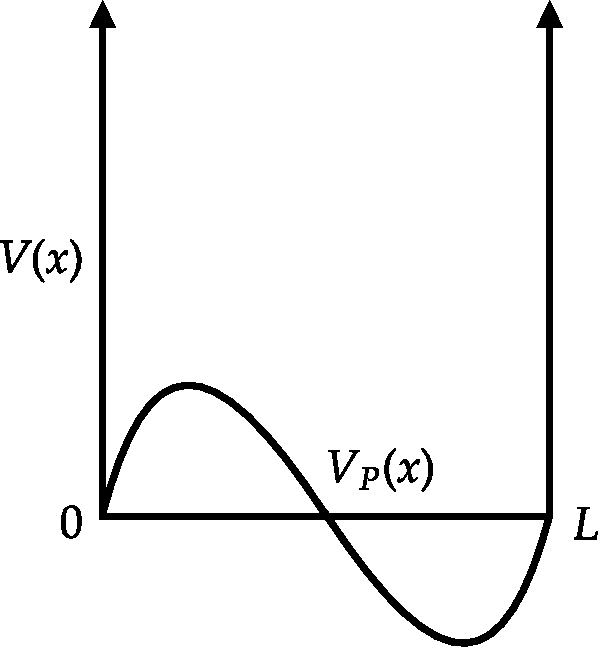
\includegraphics[height=4cm,width=4cm]{diagram-20210824-crop}
	\end{figure}
\end{minipage}
\begin{tasks}(2)
	\task[\textbf{A.}] $E^{(1)}=0 ; E^{(2)}<0$
	\task[\textbf{B.}]$E^{(1)}>0 ; E^{(2)}=0$
	\task[\textbf{C.}]$E^{(1)}=0 ; E^{(2)}$ depends on the sign of $V_{0}$
	\task[\textbf{D.}]$E^{(1)}<0 ; E^{(2)}<0$
\end{tasks}
\begin{minipage}{\textwidth}
	\item An electron with energy $E$ is incident from left on a potential barrier, given by
	$$
	V(x)= \begin{cases}0, & \text { for } x<0 \\ V_{0}, & \text { for } x>0\end{cases}
	$$
	as shown in the figure. For $E<V_{0}$, the space part of the wavefunction for $x>0$ is of the form
	\exyear{GATE 2011}
	\begin{figure}[H]
		\centering
		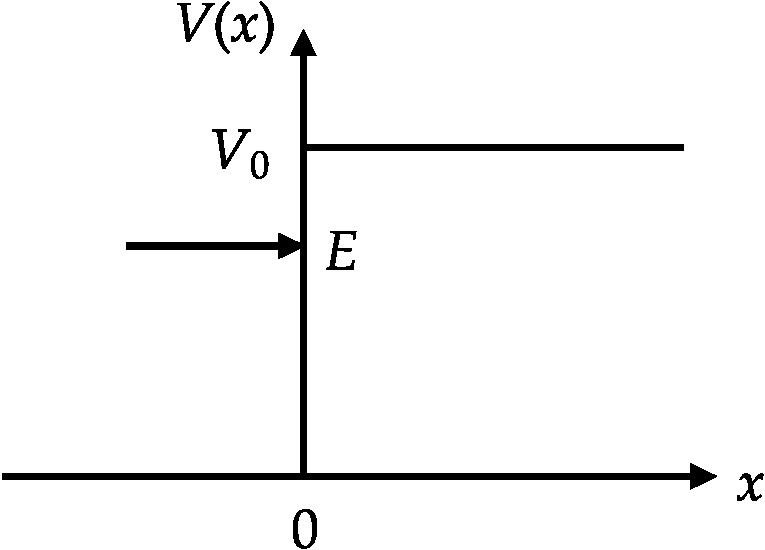
\includegraphics[height=3cm,width=5cm]{diagram-20210824(6)-crop}
	\end{figure}
\end{minipage}
\begin{tasks}(2)
	\task[\textbf{A.}] $e^{a x}$
	\task[\textbf{B.}] $e^{-a x}$
	\task[\textbf{C.}] $e^{i a x}$
	\task[\textbf{D.}]$e^{-i a x}$
\end{tasks}
\begin{minipage}{\textwidth}
	\item A particle of mass $m$ is confined in a two dimensional square well potential of dimension $a$. This potential $V(x, y)$ is given by
	$$
	\begin{aligned}
	V(x, y) &=0 \text { for }-a<x<a \text { and }-a<y<a \\
	&=\infty \text { elsewhere }
	\end{aligned}
	$$
	The energy of the first excited state for this particle is given by,
	\exyear{GATE 2012}
\end{minipage}
\begin{tasks}(2)
	\task[\textbf{A.}]$\frac{\pi^{2} \hbar^{2}}{m a^{2}}$
	\task[\textbf{B.}] $\frac{2 \pi^{2} \hbar^{2}}{m a^{2}}$
	\task[\textbf{C.}]$\frac{5 \pi^{2} \hbar^{2}}{8 m a^{2}}$
	\task[\textbf{D.}] $\frac{4 \pi^{2} \hbar^{2}}{m a^{2}}$
\end{tasks}
\begin{minipage}{\textwidth}
	\item A proton is confined to a cubic box, whose sides have length $10^{-12} \mathrm{~m}$. What is the minimum kinetic energy of the proton? The mass of proton is $1.67 \times 10^{-27} \mathrm{~kg}$ and Planck's constant is $6.63 \times 10^{-34} J_{S}$.
	\exyear{GATE 2013}
\end{minipage}
\begin{tasks}(2)
	\task[\textbf{A.}] $1.1 \times 10^{-17} \mathrm{~J}$
	\task[\textbf{B.}] $3.3 \times 10^{-17} \mathrm{~J}$
	\task[\textbf{C.}]$9.9 \times 10^{-17} \mathrm{~J}$
	\task[\textbf{D.}]$6.6 \times 10^{-17} \mathrm{~J}$
\end{tasks}
\begin{minipage}{\textwidth}
	\item Consider a system of eight non-interacting, identical quantum particles of spin $-\frac{3}{2}$ in a one dimensional box of length $L$. The minimum excitation energy of the system, in units of $\frac{\pi^{2} \hbar^{2}}{2 m L^{2}}$ is
	\exyear{GATE 2015}
\end{minipage}
\begin{minipage}{\textwidth}
	\item A two-dimensional square rigid box of side $L$ contains six non-interacting electrons at $T=0 K .$ The mass of the electron is $m .$ The ground state energy of the system of electrons, in units of $\frac{\pi^{2} \hbar^{2}}{2 m L^{2}}$ is
	\exyear{GATE 2016}
\end{minipage}
\begin{minipage}{\textwidth}
	\item A particle of mass $m$ and energy $E$, moving in the positive $x$ direction, is incident on a step potential at $x=0$, as indicated in the figure. The height of the potential is $V_{0}$, where $V_{0}>E$. At $x=x_{0}$, where $x_{0}>0$, the probability of finding the electron is $\frac{1}{e}$ times the probability of finding it at $x=0$. If $\alpha=\sqrt{\frac{2 m\left(V_{0}-E\right)}{\hbar^{2}}}$, the value of $x_{0}$ is
	\exyear{GATE 2016}
	\begin{figure}[H]
		\centering
		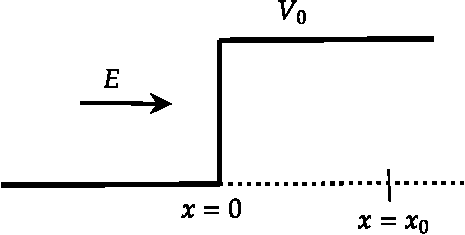
\includegraphics[height=3cm,width=5cm]{gate 5-crop}
	\end{figure}
\end{minipage}
\begin{tasks}(2)
	\task[\textbf{A.}] $\frac{2}{\alpha}$
	\task[\textbf{B.}] $\frac{1}{\alpha}$
	\task[\textbf{C.}]$\frac{1}{2 \alpha}$
	\task[\textbf{D.}]$\frac{1}{4 \alpha}$
\end{tasks}
\begin{minipage}{\textwidth}
	\item A free electron of energy $1 \mathrm{eV}$ is incident upon a one-dimensional finite potential step of height $0.75 \mathrm{eV}$. The probability of its reflection from the barrier is........... (up to two decimal places).
	\exyear{GATE 2017}
\end{minipage}
\begin{minipage}{\textwidth}
	\item The ground state energy of a particle of mass $m$ in an infinite potential well is $E_{0} .$ It changes to $E_{0}\left(1+\alpha \times 10^{-3}\right)$, when there is a small potential pump of height $V_{0}=\frac{\pi^{2} \hbar^{2}}{50 m L^{2}}$ and width $a=L / 100$, as shown in the figure. The value of $\alpha$ is (up to two decimal places).
	\exyear{GATE 2018}
\end{minipage}
\begin{minipage}{\textwidth}
	\item $ \text { Consider a potential barrier } V(x) \text { of the form: }$
	\begin{figure}[H]
		\centering
		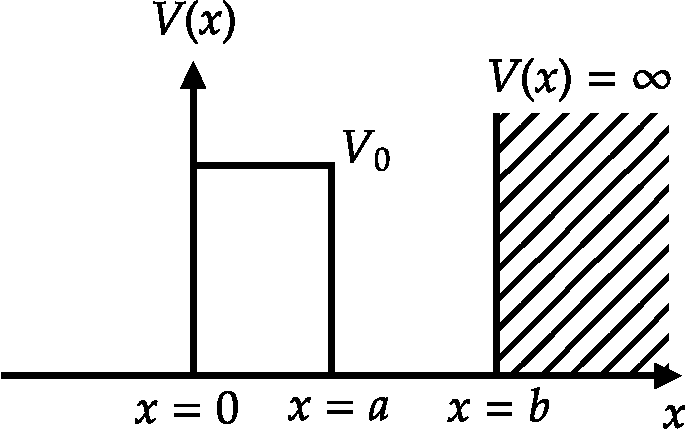
\includegraphics[height=3cm,width=5cm]{diagram-20210825(3)-crop}
	\end{figure}
	where $V_{0}$ is a constant. For particles of energy $E<V_{0}$ incident on this barrier from the left which of the following schematic diagrams best represents the probability density $|\psi(x)|^{2}$ as a function of $x$ ?
	\exyear{GATE 2019}
\end{minipage}
\begin{tasks}(2)
	\task[\textbf{A.}]\begin{figure}[H]
		\centering
		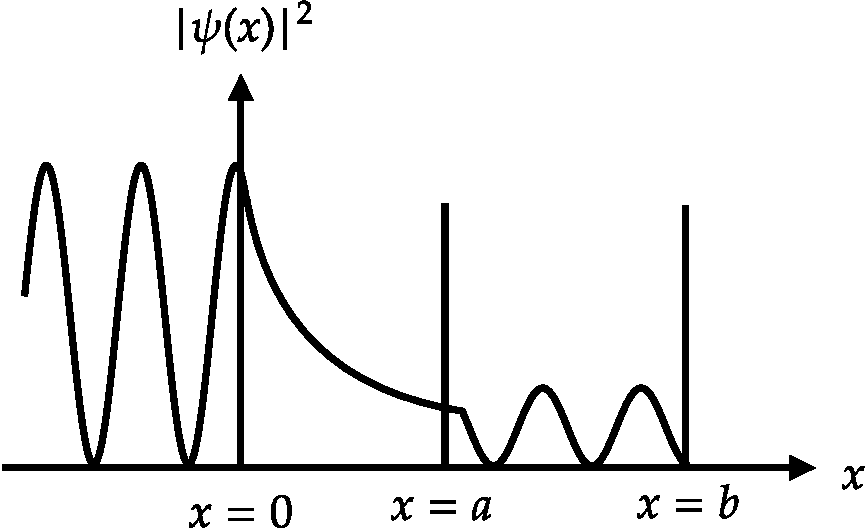
\includegraphics[height=3cm,width=5cm]{diagram-20210825(4)-crop}
	\end{figure}
	\task[\textbf{B.}]\begin{figure}[H]
		\centering
		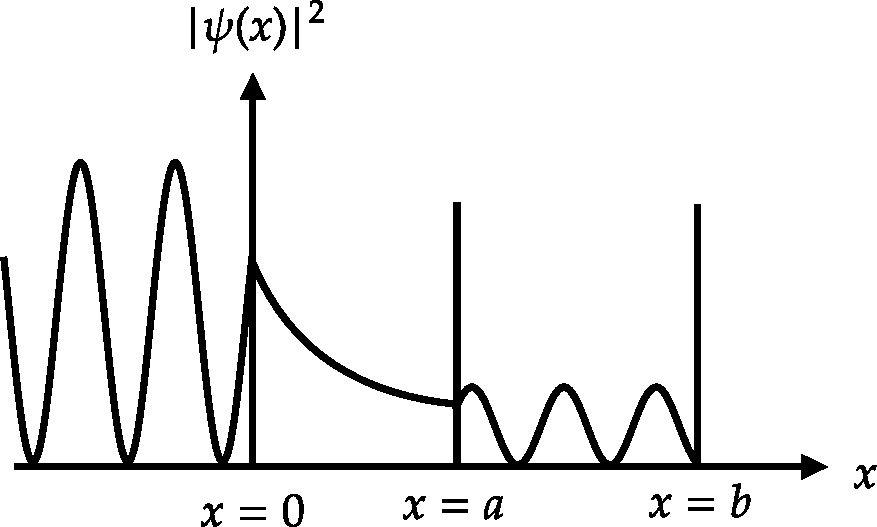
\includegraphics[height=3cm,width=5cm]{diagram-20210825(5)-crop}
	\end{figure}
	\task[\textbf{C.}]\begin{figure}[H]
		\centering
		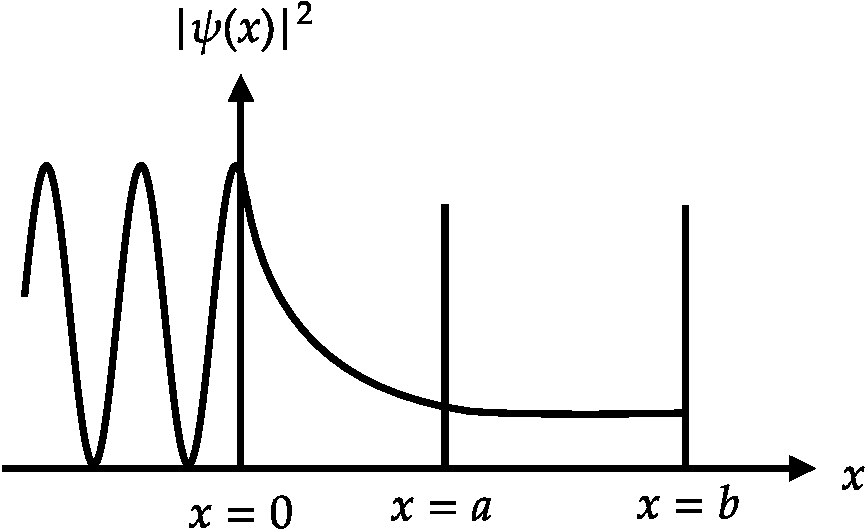
\includegraphics[height=3cm,width=5cm]{diagram-20210825(6)-crop}
	\end{figure}
	\task[\textbf{D.}]\begin{figure}[H]
		\centering
		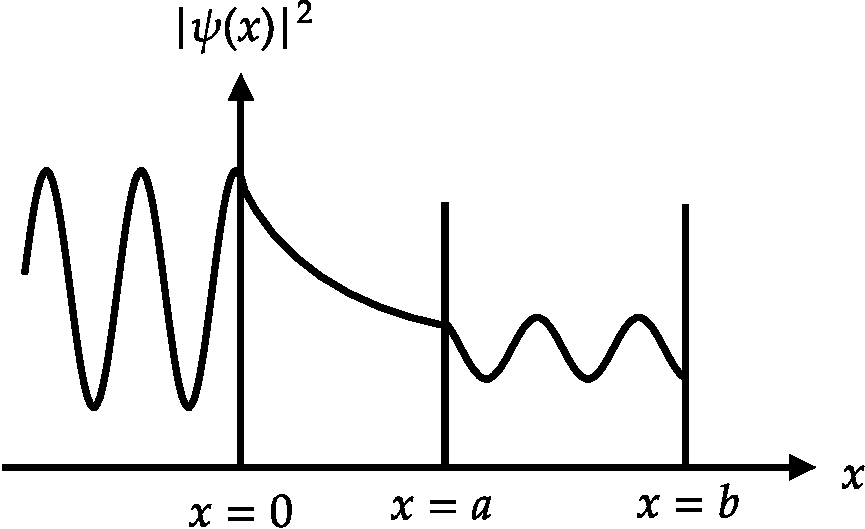
\includegraphics[height=3cm,width=5cm]{diagram-20210825(7)-crop}
	\end{figure}
\end{tasks}
\end{enumerate}


\colorlet{ocre1}{ocre!70!}
\colorlet{ocrel}{ocre!30!}
\setlength\arrayrulewidth{1pt}
\begin{table}[H]
	\centering
	\arrayrulecolor{ocre}
	
	\begin{tabular}{|p{1.5cm}|p{1.5cm}||p{1.5cm}|p{1.5cm}|}
		\hline
		\multicolumn{4}{|c|}{\textbf{Answer key}}\\\hline\hline
		\rowcolor{ocrel}Q.No.&Answer&Q.No.&Answer\\\hline
		1&\textbf{c}&2&\textbf{a}\\\hline
		3&\textbf{b}&4&\textbf{c}\\\hline
		5&\textbf{c}&6&\textbf{5}\\\hline
		7&\textbf{24}&8&\textbf{c}\\\hline
		9&\textbf{0.11}&10&\textbf{0.81}\\\hline
		11&\textbf{a}&&\\\hline
	\end{tabular}
\end{table}

\newpage
\begin{abox}
	Practice set 3
	\end{abox}
\begin{enumerate}
	\begin{minipage}{\textwidth}
	\item Consider a Hamiltonian $H=-\frac{\hbar^{2}}{2 m} \frac{d^{2}}{d x^{2}}$ and corresponding Eigen state is
	$$
	\phi_{n}(x)=\left\{\begin{array}{cc}
	\sqrt{\frac{2}{a}} \sin \frac{n \pi x}{a} & 0<x<a \\
	0 & \text { otherwise }
	\end{array}\right.
	$$
	A state $\psi(t=0)$ is defined as
	$$
	\psi=3 \phi_{1}(x)+4 \phi_{3}(x)
	$$
	(a) if energy is measured on state $\psi$ what is measurement with what probability?\\
	(b) Find $\langle E\rangle$ on state $\psi$\\
	(c) Find $\left\langle E^{2}\right\rangle$ on state $\psi$\\
	(d) Find $\Delta E . \Delta t$ on state $\psi$\\
	$\text { (e) After what time } t \psi(t=t) \text { is orthogonal to } \psi(t=0)$
\end{minipage}
\begin{answer}
	$ \psi=3 \phi_{1}(x)+4 \phi_{3}(x)$\\
	Normalised $\psi,\langle\psi \mid \psi\rangle=1$\\
	(a) measurements are $\frac{\pi^{2} \hbar^{2}}{2 m a^{2}}, \frac{9 \pi^{2} \hbar^{2}}{2 m a^{2}}$, associated with $\phi_{1}(x)$ and $\phi_{3}(x)$ with probability\\\\
	i.e. $P\left(\frac{\pi^{2} \hbar^{2}}{2 m a^{2}}\right)=\frac{\left|\left\langle\phi_{1} \mid \psi\right\rangle\right|^{2}}{\langle\psi \mid \psi\rangle}=\frac{9}{25}, P\left(\frac{9 \pi^{2} \hbar^{2}}{2 m a^{2}}\right)=\frac{\left|\left\langle\phi_{3} \mid \psi\right\rangle\right|^{2}}{\langle\psi \mid \psi\rangle}=\frac{16}{25}$\\\\
	(b) $\langle E\rangle=\sum a_{n} P\left(a_{n}\right)$ where $a_{n}$ is eigen value
	$=\frac{9}{25} \epsilon_{0}+\frac{16}{25} \times 9 \epsilon_{0}=\frac{153 \epsilon_{0}}{25} \quad$ where $\quad \frac{\pi^{2} \hbar^{2}}{2 m a^{2}}=\epsilon_{0}$\\\\
	(c) $\left\langle E^{2}\right\rangle=\sum a_{n}^{2} P\left(a_{n}\right)$
	$\frac{9}{25} \epsilon_{0}^{2}+\frac{16}{25} \times 81 \epsilon_{0}^{2}=\frac{1305}{25} \epsilon_{0}^{2}$ \\\\
	so $\Delta E=\sqrt{\left\langle E^{2}\right\rangle-\langle E\rangle^{2}}=\frac{96}{25} \epsilon_{0}$\\\\
	(d) $\Delta t=\frac{2 \pi \hbar}{\Delta E}=\frac{2 \pi \hbar}{9 \epsilon_{0}-\epsilon_{0}}=\frac{2 \pi \hbar}{8 \epsilon_{0}}$\\\\
	$\Rightarrow \Delta E . \Delta t=\frac{96}{25} \epsilon_{0} \times \frac{2 \pi \hbar}{8 \epsilon_{0}}=\frac{12 h}{25}$
	\begin{align*}
		&\text { (e) }|\psi(x, t)\rangle=\frac{3}{5} \phi_{1}(x) e^{\frac{-i \epsilon_{0} t}{\hbar}}+\frac{4}{5} \phi_{3}(x) e^{\frac{-i \theta_{0} t}{\hbar}} \\
		&\text { now }\langle\psi(x, 0) \mid \psi(x, t)\rangle=0 \Rightarrow \frac{9}{25} e^{\frac{-i \epsilon_{0} t}{\hbar}}+\frac{16}{25} e^{\frac{-\frac{-19 \epsilon_{0} t}{\hbar}}{\hbar}}=0 \\
		&\Rightarrow \frac{16}{25} e^{\frac{-19 \epsilon_{0} t}{h}}=-\frac{9}{25} e^{\frac{-i \epsilon_{0} t}{\hbar}} \Rightarrow \cos \frac{\left(9 \varepsilon_{0}-\epsilon_{0}\right) t}{\hbar}=\frac{-9}{16} \\
		&\Rightarrow t=\frac{\hbar}{8 \epsilon_{0}} \cos ^{-1} \frac{-9}{16} \Rightarrow t=\frac{m a^{2}}{4 \pi^{2} \hbar} \cos ^{-1}\left(\frac{-9}{16}\right)
	\end{align*}
\end{answer}
	\begin{minipage}{\textwidth}
	\item A particle in the infinite well has initial wave function
	$$
	\psi(x, 0)= \begin{cases}A x(a-x) ; & (0 \leq x<a) \\ 0 ; & \text { otherwise }\end{cases}
	$$
	If Eigen state of system is given by
	$$
	\phi_{n}= \begin{cases}\sqrt{\frac{2}{a}} \sin \frac{n \pi x}{a} ; & 0<x<a \\ 0 & ; \quad \text { otherwise }\end{cases}
	$$
	and if normalized $\psi(x, 0)$ is defined as $\psi(x, 0)=c_{1} \phi_{1}(x)+c_{2} \phi_{2}(x)+c_{3} \phi_{3}(x)$, then find the value of $c_{1}, c_{2}$ and $c_{3} .$
\end{minipage}
\begin{answer}
	$\text { Normalization of } \psi \Rightarrow\langle\psi \mid \psi\rangle=1 \Rightarrow \int_{0}^{a} A^{2} x^{2}(a-x)^{2} d x=1 \quad \Rightarrow \quad A=\sqrt{\frac{30}{a^{5}}}$\\
	\begin{align*}
		&\psi(x, 0)=c_{1} \phi_{1}(x)+c_{2} \phi_{2}(x)+c_{3} \phi_{3}(x) \\
		&\Rightarrow c_{1}=\left\langle\phi_{1} \mid \psi\right\rangle, c_{2}=\left\langle\phi_{2} \mid \psi\right\rangle, \quad c_{3}=\left\langle\phi_{3} \mid \psi\right\rangle\\
		&\text { now } c_{1}=\left\langle\phi_{1} \mid \psi\right\rangle=\int_{0}^{a} \sqrt{\frac{30}{a^{5}}} \sqrt{\frac{2}{a}}\left(a x-x^{2}\right) \sin \frac{\pi x}{a} d x \\
		&=\sqrt{\frac{60}{a^{6}}}\left[\int_{0}^{a} a x \frac{\sin \pi x}{a} d x-\int_{0}^{a} x^{2} \sin \frac{\pi x}{a} d x\right] \\
		&\Rightarrow c_{1}=\sqrt{\frac{60}{a^{6}}}\left[-\frac{2 a^{3}}{\pi^{3}} \cos \left(\frac{\pi x}{a}\right)\right]_{0}^{a} \Rightarrow c_{1}=\frac{4 a^{3}}{\pi^{3}} \times \sqrt{\frac{60}{a^{6}}}=0.99807\\
		&c_{2}=\left\langle\phi_{2} \mid \psi\right\rangle=\int_{0}^{a} \sqrt{\frac{30}{a^{5}}}\left(a x-x^{2}\right) \sqrt{\frac{2}{a}} \sin \left(\frac{2 \pi x}{a}\right) d x \\
		&=\sqrt{\frac{60}{a^{6}}}\left[\int_{0}^{a} a x \sin \left(\frac{2 \pi x}{a}\right) d x-\int_{0}^{a} x^{2} \sin \left(\frac{2 \pi x}{a}\right) d x\right] \\
		&=\sqrt{\frac{60}{a^{6}}}\left[-\frac{a^{2}}{2 \pi^{2}}(1-1)\right]=0 \Rightarrow c_{2}=0\\
		&c_{3}=\left\langle\phi_{3} \mid \psi\right\rangle=\int_{0}^{a} \sqrt{\frac{30}{a^{5}}} \sqrt{\frac{2}{a}}\left(a x-x^{2}\right) \sin \left(\frac{3 \pi x}{a}\right) d x \\
		&=\sqrt{\frac{60}{a^{6}}}\left[\int_{0}^{a} a x \sin \left(\frac{3 \pi x}{a}\right) d x-\int_{0}^{a} x^{2} \sin \left(\frac{3 \pi x}{a}\right) d x\right] \\
		&=\sqrt{\frac{60}{a^{6}}}\left[\frac{4 a^{3}}{27 \pi^{3}}\right]=0.036965 \Rightarrow c_{3}=0.0369
	\end{align*}
\end{answer}
	\begin{minipage}{\textwidth}
	\item A particle of mass $m$ is confined to one-dimensional region $0 \leq x \leq a$ where potential is given by
	$$
	V(x)= \begin{cases}\infty ; & x \leq 0, \quad x \geq a \\ 0 ; & 0<x<a\end{cases}
	$$
	Its normalized wave function is given by
	$$
	\psi(x, t=0)=\sqrt{\frac{8}{5 a}}\left[1+\cos \frac{\pi x}{a}\right] \sin \frac{\pi x}{a}
	$$
	(a) What is the wave function at a later time $t=t_{0}$\\
	(b) What is the average energy of the system at $t=0$ and $t=t_{0}$.\\
	(c) What is the probability that the particle is found in the left half of the box at $t=0$\\
	(d) Find $\langle x\rangle$ on state $\psi$ at $t=0$
\end{minipage}
\begin{answer}
$\psi(x, t=0)=\sqrt{\frac{8}{5 a}}\left[1+\cos \left(\frac{\pi x}{a}\right)\right] \sin \left(\frac{\pi x}{a}\right)$\\
$=\sqrt{\frac{8}{5 a}} \sin \left(\frac{\pi x}{a}\right)+\sqrt{\frac{8}{5 a}} \cos \frac{\pi x}{a} \cdot \sin \frac{\pi x}{a}=\sqrt{\frac{4}{5}} \sqrt{\frac{2}{a}} \sin \frac{\pi x}{a}+\frac{1}{\sqrt{5}} \sqrt{\frac{2}{a}} \sin \left(\frac{2 \pi x}{a}\right)$\\
$\psi(x, 0)=\sqrt{\frac{4}{5}} \phi_{1}(x)+\frac{1}{\sqrt{5}} \phi_{2}(x)$\\
(a) $\psi\left(x, t=t_{0}\right)=\sqrt{\frac{4}{5}} \phi_{1}(x) e^{\frac{-i \epsilon_{0} t_{0}}{\hbar}}+\frac{1}{\sqrt{5}} \phi_{2}(x) e^{\frac{-i 4 \epsilon_{0} t_{0}}{\hbar}}$
$$
\left(\because \in_{0}=\frac{\pi^{2} \hbar^{2}}{2 m a^{2}}\right)
$$
$\text { (b) }\langle E\rangle=\sum a_{n} p\left(a_{n}\right)$\\\\
i.e. $P\left(\epsilon_{0}\right)=\frac{\left|\left\langle\phi_{1} \mid \psi\right\rangle\right|^{2}}{\langle\psi \mid \psi\rangle}=\frac{4}{5}$\\\\
 and $P\left(4 \epsilon_{0}\right)=\frac{\left|\left\langle\phi_{2} \mid \psi\right\rangle\right|^{2}}{\langle\psi \mid \psi\rangle}=\frac{1}{5} \Rightarrow\langle E\rangle=\frac{4}{5} \times \epsilon_{0}+\frac{1}{5} \times 4 \in_{0}=\frac{8}{5} \epsilon_{0}$\\\\
 and $\psi\left(x, t=t_{0}\right)=\sqrt{\frac{4}{5}} \phi_{1} \in_{0} e^{\frac{-i \epsilon_{0} t}{\hbar}}+\frac{1}{\sqrt{5}} \phi_{2} e^{\frac{-i 4 \epsilon_{0} t}{\hbar}}$\\\\
Probability of getting $\epsilon_{0}$ and $4 \epsilon_{0}$ are $\frac{4}{5}$ and $\frac{1}{5}$ respectively and $\langle E\rangle=\frac{8 \epsilon_{0}}{5}$.\\
(c) probability that particle will in first half of box
$$
\begin{gathered}
\int_{0}^{\frac{a}{2}}|\psi|^{2} d x \Rightarrow \int_{0}^{\frac{a}{2}} \frac{4}{5}\left|\phi_{1}\right|^{2} d x+\frac{1}{5} \int_{0}^{\frac{a}{2}}\left|\phi_{2}\right|^{2} d x+2 \cdot \sqrt{\frac{4}{5}} \cdot \frac{1}{\sqrt{5}} \int_{0}^{\frac{a}{2}} \phi_{1} \phi_{2} d x \\
\Rightarrow \frac{4}{5} \cdot \frac{1}{2}+\frac{1}{5} \cdot \frac{1}{2}+\frac{4}{5 a} \int_{0}^{\frac{a}{2}} 2 \sin \frac{\pi x}{a} \cdot \sin \frac{2 \pi x}{a} d x \Rightarrow \frac{1}{2}+\frac{4}{5 a}\left[\int_{0}^{\frac{a}{2}}\left[\cos \left(\frac{\pi x}{a}\right)-\cos \left(\frac{3 \pi x}{a}\right) d x\right]\right] \\
\Rightarrow \frac{1}{2}+\frac{4}{5 a}\left\{\frac{a}{\pi}+\frac{a}{3 \pi}\right\} \Rightarrow \frac{1}{2}+\frac{16}{15 \pi}
\end{gathered}
$$
(d) $\langle x\rangle=\frac{\langle\psi|X| \psi\rangle}{\langle\psi \mid \psi\rangle}=\frac{4}{5}\left\langle\phi_{1}|x| \phi_{1}\right\rangle+\frac{1}{5}\left\langle\phi_{2}|x| \phi_{2}\right\rangle+2 \sqrt{\frac{4}{5}} \frac{1}{\sqrt{5}} \int_{0}^{a} \phi_{1}^{*} x \phi_{2} d x$\\\\ $\Rightarrow\langle x\rangle=\frac{4}{5} \cdot \frac{a}{2}+\frac{1}{5} \cdot \frac{a}{2}+\frac{4}{5 a} \int_{0}^{a}\left[x \cos \frac{\pi x}{a}-x \cos \frac{3 \pi x}{a}\right] d x$
\begin{align*}
&\Rightarrow\langle x\rangle=\frac{a}{2}+\frac{4}{5 a}\left[\frac{a}{\pi} \frac{\cos \frac{x}{a}}{\frac{\pi}{a}}-\frac{3 \pi}{a} \frac{\cos \frac{3 \pi x}{a}}{\frac{3 \pi}{a}}\right]_{0}^{a} \\
&\Rightarrow\langle x\rangle=\frac{a}{2}+\frac{4}{5 a}\left[\frac{a^{2}}{\pi^{2}}(-1-1)-\frac{a^{2}}{9 \pi^{2}}(-1-1)\right] \Rightarrow\langle x\rangle=\frac{a}{2}-\frac{64 a}{45 \pi^{2}}
\end{align*}	
\end{answer}
	\begin{minipage}{\textwidth}
	\item Particles of energy $9 \mathrm{eV}$ are sent towards a potential step $8 \mathrm{eV}$ high. What percentage of particles will reflect back?
\end{minipage}
\begin{answer}
	$\left(\frac{\sqrt{E}-\sqrt{E-V_{0}}}{\sqrt{E}+\sqrt{E-V_{0}}}\right)^{2}=\left(\frac{\sqrt{9}-\sqrt{1}}{\sqrt{9}+\sqrt{1}}\right)^{2}=\frac{1}{4}$\\\\
	$\text { So, } 25 \% \text { of the particles will reflect back. }$
\end{answer}
	\begin{minipage}{\textwidth}
	\item Electrons of $1 \mathrm{eV}$ are incident on a barrier of height $10 \mathrm{eV}$ and width $0.5 \mathrm{~nm} .$ Find the transmission probability. What will be the probability if the particle is proton instead of electron?
\end{minipage}
\begin{answer}
	$\text { We have } \gamma=\sqrt{\frac{2 m\left(V_{0}-E\right)}{\hbar^{2}}}=\sqrt{\frac{9 \mathrm{eV}}{38 \times 10^{-3} \mathrm{eVnm}^{2}}} \approx 15 \mathrm{~nm}^{-1}$\\
	$\text { or, } \quad 2 \gamma L=2 \times 15 \times 0.5=15$\\
	As it is quite large as compared to 1 , one can use the approximation
	$$
	T: \approx e^{-2 \gamma L}=e^{-15} \approx 3 \times 10^{-7}
	$$
	If the particle is a proton,
	$$
	\gamma=\sqrt{\frac{1836 m_{e}\left(V_{0}-E\right)}{\hbar^{2}}}=\sqrt{1836} \times 15 \mathrm{~nm}^{-1}=643 \mathrm{~nm}^{-1} .
	$$
	For $2 \gamma L \approx 643$, the transmission probability
	$$
	T=e^{-2 \gamma L}=e^{-643} \approx 10^{-279} .
	$$
\end{answer}
	\begin{minipage}{\textwidth}
	\item A particle of mass $m$ moves in the potential $V(x)=\frac{1}{2} m \omega^{2} x^{2} .$ It has wave function $\psi(x)$ at time $t=0$. What will be the wave function at time, $t=2 \pi / \omega$ (one time period)?
\end{minipage}
\begin{answer}
	Let the wave function at $t=0$ be $\psi(x)=\sum_{n} C_{n}\left|\phi_{n}\right\rangle$\\
	The wave function at time $t$ will be
	$$
	\psi(x, t)=\sum_{n} C_{n}\left|\phi_{n}\right\rangle e^{-\frac{i}{\hbar} E_{n t}}=\sum_{n} C_{n}\left|\phi_{n}\right\rangle e^{-\frac{i}{\hbar}\left(n+\frac{1}{2}\right) h\omega t}
	$$
	$$=\sum_{n} C_{n}\left|\phi_{n}\right\rangle e^{-i\left(n+\frac{1}{2}\right) 2 \pi}=\sum_{n} C_{n}\left|\phi_{n}\right\rangle e^{-i \pi}=\sum_{n} C_{n}\left|\phi_{n}\right\rangle=-\psi(x)$$
	In one time period the wave function becomes negative of its original form. In two time periods, it regains its original shape.
\end{answer}
	\begin{minipage}{\textwidth}
	\item A quantum mechanical particle in a harmonic oscillator potential with potential $\frac{1}{2} m \omega^{2} x^{2}$ has the initial wave function $\psi=\phi_{0}(x)+\phi_{1}(x)$, where $\phi_{0}$ and $\phi_{1}$ are the real wave functions in the ground and first excited state of the harmonic oscillator Hamiltonian.\\
	(a) Find the average value of energy on state $\psi=\phi_{0}(x)+\phi_{1}(x)$,\\
	(b) Find average value of $X$ on state $\psi$.\\
	(c) Find average value of $X^{2}$ on state $\psi$
\end{minipage}
\begin{answer}
$\text { (a) If energy is measured on state } \psi \text { the measurement is } \frac{\hbar \omega}{2} \text { and } \frac{3 \hbar \omega}{2} \text { with }$\\
probability $\frac{1}{2}$ for each measurement .\\\\
$\langle E\rangle=\frac{1}{2}\left(\frac{\hbar \omega}{2}\right)+\frac{1}{2}\left(\frac{3 \hbar \omega}{2}\right)=\hbar \omega$\\\\
$\text { (b) }|\psi\rangle=\frac{1}{\sqrt{2}}\left(\left|\phi_{0}\right\rangle+\left|\phi_{1}\right\rangle\right)$\\
$\left|\phi_{0}\right\rangle=\left(\frac{m \omega}{\pi \hbar}\right)^{1 / 4} e^{\frac{-m \omega x^{2}}{2 \hbar}} \quad \text { and }\left|\phi_{1}\right\rangle=\left(\frac{m \omega}{\pi \hbar}\right)^{1 / 4} \cdot \sqrt{2} \cdot\left(\frac{m \omega}{\hbar}\right)^{1 / 2} \cdot x . e^{\frac{-m \omega x^{2}}{2 \hbar}},\langle\psi \mid \psi\rangle=1$\\\\
$\langle X\rangle=\frac{1}{2}\left\langle\phi_{0}|X| \phi_{0}\right\rangle+\frac{1}{2}\left\langle\phi_{1}|X| \phi_{1}\right\rangle+\left\langle\phi_{0}|X| \phi_{1}\right\rangle ; \quad\left\langle\phi_{0}|X| \phi_{0}\right\rangle=0,\left\langle\phi_{1}|X| \phi_{1}\right\rangle=0$\\\\
$\left\langle\phi_{0}|X| \phi_{1}\right\rangle=\left(\frac{m \omega}{\pi \hbar}\right)^{1 / 2} \cdot \sqrt{2}\left(\frac{m \omega}{\hbar}\right)^{1 / 2} \cdot \int_{-\infty}^{\infty} x^{2} e^{\frac{-m \omega x^{2}}{\hbar}} d x=\frac{1}{\sqrt{2}}\left(\frac{m \omega}{\hbar}\right)\left(\frac{\hbar}{m \omega}\right)^{3 / 2}=\sqrt{\frac{\hbar}{2 m \omega}}$\\\\
$$\langle X\rangle=\sqrt{\frac{\hbar}{2 m \omega}}$$
(c) $\left\langle X^{2}\right\rangle=\frac{1}{2}\left\langle\phi_{0}\left|X^{2}\right| \phi_{0}\right\rangle+\frac{1}{2}\left\langle\phi_{1}\left|X^{2}\right| \phi_{1}\right\rangle+\frac{1}{2}\left\langle\phi_{0}\left|X^{2}\right| \phi_{1}\right\rangle+\frac{1}{2}\left\langle\phi_{1}\left|X^{2}\right| \phi_{0}\right\rangle$\\\\
$\left\langle\phi_{0}\left|X^{2}\right| \phi_{1}\right\rangle=0,\left\langle\phi_{1}\left|X^{2}\right| \phi_{0}\right\rangle=0$	\\\\
\begin{align*}
	&\left\langle\phi_{0}\left|X^{2}\right| \phi_{0}\right\rangle=\left(\frac{m \omega}{\pi \hbar}\right)^{1 / 2} \int_{-\infty}^{\infty} x^{2} \cdot e^{\frac{-m \omega x^{2}}{\hbar}} d x=\left(\frac{m \omega}{\pi \hbar}\right)^{1 / 2}\left(\frac{\hbar}{m \omega}\right)^{3 / 2} \times \frac{1}{2} \sqrt{\pi}=\left(\frac{\hbar}{2 m \omega}\right) \\
	&\left\langle\phi_{1}\left|X^{2}\right| \phi_{1}\right\rangle=\left(\frac{m \omega}{\pi \hbar}\right)^{1 / 2}(\sqrt{2})^{2}\left(\frac{m \omega}{\hbar}\right) \int_{-\infty}^{\infty} x^{4} e^{\frac{-m \omega x^{2}}{\hbar}} d x=\frac{3}{2}\left(\frac{\hbar}{m \omega}\right)
\end{align*}

$$\text { Hence }\left\langle X^{2}\right\rangle=\left(\frac{\hbar}{4 m \omega}\right)+\frac{3}{4}\left(\frac{\hbar}{m \omega}\right)=\left(\frac{\hbar}{m \omega}\right)$$
\end{answer}
	\begin{minipage}{\textwidth}
	\item A Particle of mass in harmonic oscillator potential starts out in state $\psi(x, 0)=A\left[3 \psi_{0}(x)+4 \psi_{1}(x)\right] .$ Where $\psi_{0}$ is ground state and $\psi_{1}$ is first excited state.\\
	(a) Find $A$\\
	(b) construct $\psi(x, t)$ and $|\psi(x, t)|^{2}$\\
\end{minipage}
\begin{answer}
	$\text { (a) } \psi(x, 0)=A\left[3 \psi_{0}(x)+4 \psi_{1}(x)\right]$\\\\
	$\text { From normalization condition } A=\frac{1}{\sqrt{9+16}}=\frac{1}{5}$\\
(b)	\begin{align*}
		&\psi(x, 0)=\frac{3}{5} \psi_{0}(x)+\frac{4}{5} \psi_{1}(x) \\
		&\psi(x, t)=\frac{3}{5} \psi_{0}(x) e^{-\frac{\hbar \omega e r}{2 \hbar}}+\frac{4}{5} \psi_{1} e^{-i \frac{3 h \omega t}{2 \hbar}} \\
		&\quad=\frac{3}{5} \psi_{0}(x) e^{\frac{-i \omega t}{2}}+\frac{4}{5} \psi_{1} e^{-\frac{i 3 \omega t}{2}} \\
		&|\psi(x, t)|^{2}=\frac{9}{25}\left|\psi_{0}\right|^{2}+\frac{16}{25}\left|\psi_{1}\right|^{2}+2 \times \frac{3}{5} \times \frac{4}{5} \psi_{0} \psi_{1} \cos \left(\frac{3 \hbar \omega}{2}-\frac{\hbar \omega}{2}\right) t / h \\
		&\quad=\frac{9}{25}\left|\psi_{0}\right|^{2}+\frac{16}{25}\left|\psi_{1}\right|^{2}+\frac{24}{25} \psi_{0} \psi_{1} \cos \omega t
	\end{align*}
\end{answer}
\end{enumerate}











